\graphicspath{{Dissertation/images/chapt1/}}


\chapter{Сдвиг положения ядра с частотой в ультракомпактных квазарах} \label{chapt1}


\section{Введение}
На изображениях внегалактических релятивистских струй, полученных с помощью Радиоинтерферометрии со
СверхДлинными Базами (РСДБ), ``ядром'' обычно называют наиболее компактную и яркую деталь у видимого
основания струи. Положение ядра определяется поглощением в излучающей плазме (синхротронное
самопоглощение) или поглощением в окружающем веществе
\cite{Blandford_Konigl_1979,Konigl_1981,Lobanov_1998}. На частоте наблюдения $\nu$ ядро находится в
области струи с оптической толщей $\tau(\nu) \approx 1$, что приводит к смещению абсолютного
положения ядра $r_\mathrm{core}$ как $\propto \nu^{-1/k_{\mathrm{r}}}$ \cite{Lobanov_1998}. В случае
синхротронного самопоглощения и при равнораспределении плотности энергии частиц и магнитного поля
$k_\mathrm{r} = 1$ \cite{Blandford_Konigl_1979}. Однако при наличии внешнего поглощения или
градиентов плотности и давления, $k_\mathrm{r}$ может отличаться от единицы \cite{Lobanov_1998}.

Эффект видимого сдвига ядра активных ядер галактик имеет непосредственные астрофизические и
астрометрические приложения в исследованиях компактных радиоисточников. Этот эффект может быть
использован для оценок
различных физических параметров компактных релятивистских струй. С другой стороны, сдвиг ядра с
частотой может влиять на измерения и оценки, основанные на многочастотных РСДБ наблюдениях: 1)
построение карт спектрального индекса \cite{Lobanov_1998,Kovalev_2008}; 2) измерения фарадеевского
вращения \cite{Hovatta_2012,Krav2016,Krav2017}; 3) астрометрические и геофизические измерения в
диапазонах 4 и 13~см \cite{Ma_1998,Petrov2009}; 4) сопоставление радио и оптической системы
координат \cite{PK_letter2017,KPP2017,PK2017}.

Для понимания и учета эффектов поглощения в подобных исследованиях необходимо систематическое
изучение смещения ядра, которое бы охватывало репрезентативную выборку компактных радиоисточников, в
частности, тех, которые используются в астрометрических приложениях. Для достижения этой цели мы
организовали пилотный эксперимент на Европейской РСДБ сети. Он преследовал следующие цели:
проведение измерений сдвига ядра у ультракомпактных квазаров методом относительной астрометрии в
рамках отобранных триплетов источников, сравнение результатов с традиционным методом
привязки к оптически тонким частям струи самого источника, получение опыта для использования в
организации более массовых астрометрических измерений данного эффекта в будущем, апробация участия
российской системы Квазар-КВО в наблюдениях Европейской РСДБ сети и оценка выигрыша от такого
участия.

\section{Наблюдения и обработка данных}

\subsection{Выборка источников}
Для наблюдений мы отобрали восемь ультракомпактных внегалактических радиоисточников, которые
соответствуют следующим критериям: 1) источник входит в основной список объектов каталога ICRF
\cite{Ma_1998}; 2) структурный индекс источника равен 1 или 2 \cite{Ma_1998}, то есть в структуре
источника доминирует ядро; 3) максимальная коррелированная спектральная плотность потока источника
на частоте 8~ГГц больше 1.2~Ян. На основе этих критериев мы также добавили источник 1749+096,
который является самым компактным и ярким объектом из списка кандидатов в каталог ICRF
\cite{Ma_1998}. Для каждого такого источника мы подобрали по два фазовых калибратора на угловом
расстоянии не больше $4^\circ$.

\subsection{EVN наблюдения}
Наблюдения выбранных источников проводились на Европейской РСДБ-сети (European VLBI Network, EVN) в
рамках трех 12-часовых сессий в октябре 2008 года: 19--20 октября в частотных диапазонах S/X
(центральная частота 2.27 и 8.38~ГГц), 22--23 октября в диапазоне C (4.97~ГГц) и 29--30 октября в
диапазоне L (1.66~ГГц).
В каждом диапазоне записывалось по 8 частотных каналов (IF) шириной 8 МГц каждый. В диапазонах L и C
записывались правая и левая круговые поляризации, в то время как в диапазонах S и X~--- только
правая. Суммарный битовый поток составил 512 Мбит/с. Корреляция данных была произведена в
JIVE (Joint Institute for VLBI in Europe).

В этом эксперименте в наблюдениях EVN впервые принимали участие три 32-метровых телескопа российской
РСДБ-сети ``Квазар-КВО'', что заметное улучшило покрытие плоскости пространственных частот в
направлении восток-запад (см. раздел \ref{s:kvazar}). Однако, поломка телескопа в обсерватории
Hartebeesthoek в Южной Африке заметно ограничила разрешение интерферометрической сети в направлении
север-юг. К сожалению, это драматическим образом повлияло на точность астрометрических измерений
данного проекта, так как именно базы интерферометра с участием  антенны Hartebeesthoek должны были
предоставить наиболее высокое угловое разрешение а данных измерениях.

\subsection{Обработка данных}
Первичная обработка данных проводилась в программном пакете \emph{AIPS} \cite{Greisen_2003} и
включала в себя следующие этапы: исключение плохих данных на основе сообщений с телескопов и
визуальной инспекции данных; применение коррекций фазы, связанных с прохождением радиосигнала через
ионосферу при помощи задачи \emph{TECOR}; калибровка амплитуды с использованием системных
температур и кривых усиления, измеренных на телескопах, при помощи задачи \emph{APCAL}; первичная
калибровка фазы при помощи процедуры глобальной подгонки лепестков (задача \emph{FRING}). Для
каждого частотного канала (IF) находилось независимое решение для групповой задержки и частоты
интерференции. Форма комплексной полосы пропускания исправлялась при помощи задачи
\emph{BPASS}. Далее, с помощью задачи \emph{SPLIT} все найденные поправки применялись к данным, и
после усреднения по частоте в пределах каждого IF, UV-данные экспортировались в формате, пригодном
для дальнейшего анализа.

Для всех источников были построены карты с использованием алгоритма CLEAN, реализованного в
программе {\em Difmap} \cite{Shepherd_1997}. Для каждого частотного канала каждой антенны
были получены глобальные поправки амплитуды путем сравнения полной интенсивности CLEAN модели с
изначальными калиброванными данными. Полученные поправки усреднялись по всем источникам.
Поправки амплитуды >10\% затем вводились в исходные данные с помощью задачи \emph{CLCOR} в
\emph{AIPS}.

Финальная обработка данных в \emph{AIPS} проводилась в режиме фазовой привязки более слабых
источников триплета к калибратору. Для этого в каждом триплете выбирался наиболее яркий и
компактный источник в качестве фазового калибратора. Далее для каждого калибратора находилось
фазовое решение с помощью задачи \emph{FRING} с учетом его структуры, которое затем применялось как
к данным самого калибратора, так и к данным двух других источников данного триплета.

\subsection{Восстановленные РСДБ карты}

Финальные РСДБ изображения 24 наблюдаемых источников с использованием натурального взвешивания
данных приведены на рис.~\ref{fig:maps}. Для каждого источника мы представляем контурные карты на
частотах 1.7, 2.3, 5.0 и 8.4~ГГц. Динамический диапазон карт, определяемый как отношение пика
интенсивности изображения к уровню остаточного шума карты, варьируется от $10^3$ для слабых
источников до $10^4$ для самых ярких на частотах 1.7, 5.0 и 8.4~ГГц. Для карт
на частоте 2.3~ГГц динамический диапазон карт ниже, особенно для источников слабее 1~Ян, поскольку в
наблюдениях на данной частоте не принимала участие фазированная антенная решетка Westerbork,
являвшаяся одним из самых чувствительных элементов европейской РСДБ сети. Типичный уровень шума
восстановленных изображений составляет 0.3~мЯн/луч.

В таблице~\ref{tab:maps} мы суммируем параметры РСДБ карт: название источника, центральная частота
синтезированного изображения в ГГц, пик интенсивности в мЯн/луч, уровень остаточного шума в
мЯн/луч, полный поток с карты в мЯн как сумма потоков всех CLEAN компонентов, размеры большой и
малой оси диаграммы направленности по уровню половинной мощности в миллисекундах дуги, позиционный
угол большой оси диаграммы в градусах.

\subsection{Моделирование источников}
\label{s:modeling}
Для того чтобы определить положение ядра на карте, мы моделировали распределение яркости каждого
источника набором круговых гауссовых компонентов. Подгонка модели к данным производилась в области
пространственных частот в программе \emph{Difmap} путем минимизации $\chi^2$. Количество компонентов
выбиралось минимально достаточным (обычно 3--6) для описания всех значимо продетектированных
элементов структуры источника на данной частоте.

\subsection{Значимость сети ``Квазар-КВО'' для получаемых результатов измерений Европейской РСДБ
сети}
\label{s:kvazar}
Как показано на рис.~\ref{fig:uv}, телескопы российского радиоинтерферометрического комплекса
``Квазар-КВО'' значительно улучшают заполнение UV-плоскости сети EVN, особенно на средних базах.
Участие трех антенн сети ``Квазар'' в дополнение к восьми EVN-станциям увеличивает количество
баз интерферометра примерно в два раза, что повышает надежность восстанавливаемого изображения и
значимо уменьшает уровень шума.
Чтобы оценить, какой вклад вносят данные телескопов сети ``Квазар'', мы провели полную переобработку
данных, исключив телескопы Бадары, Зеленчук и Светлое, и построили карты трех источников 0125+487,
0133+476 и 0151+474 на всех частотах. Мы выбрали для данного анализа источники с высоким
склонением, чтобы уменьшить влияние плохого заполнения UV-плоскости в направлении север-юг. На
рис.~\ref{fig:map_rms} приведен график, который позволяет сравнить уровень остаточного шума
изображений, восстановленных с использование данных телескопов сети ``Квазар'' и без них. Во втором
случае уровень остаточного шума изображений оказывается в среднем выше на 30\%. В тоже время,
остаточный шум изображений источника 0151+474 в диапазонах L, C и X остался практически неизменным.
Отсутствие дополнительных интерферометрических баз особенно критически может сказаться на
восстановлении изображений слабых источников, протяженная структура которых не будет
продетектирована из-за недостаточной  чувствительности интерферометра.

\subsection{Калибровка фазы}
Фаза функции видности на выходе коррелятора представляет собой сумму вкладов различных эффектов:
\[
 \varphi = \varphi_\mathrm{struct} + \varphi_\mathrm{pos} + \varphi_\mathrm{atmo} +
\varphi_\mathrm{inst} \, \text{,}
\]
где $\varphi_\mathrm{struct}$~--- фаза, связанная со структурой источника;
$\varphi_\mathrm{pos}$~--- фаза, связанная с несовпадением координат источника и фазового центра;
$\varphi_\mathrm{atmo}$~--- влияние атмосферы (ионосфера и тропосфера); $\varphi_\mathrm{inst}$~---
фаза, связанная с задержками в аппаратуре и неидеальностью стандартов частоты.

Слагаемые $\varphi_\mathrm{struct}$ и $\varphi_\mathrm{pos}$ определяются источником, в то время
как слагаемые $\varphi_\mathrm{atmo}$ и $\varphi_\mathrm{inst}$ связаны с телескопами. Процедура
глобальной подгонки лепестков минимизирует фазу, вводя глобальные поправки для антенн. Таким
образом определяется сумма $\varphi_\mathrm{atmo} + \varphi_\mathrm{inst} + \varphi_\mathrm{pos}$.
Остается только слагаемое, которое зависит от проекции интерференционной базы (UV координат)~---
$\varphi_\mathrm{struct}$.

После калибровки с фазовым калибратором, фаза целевого источника будет следующая:
\[
 \varphi^{t} = \varphi_\mathrm{struct}^\mathrm{t} + (\varphi_\mathrm{pos}^\mathrm{t} -
\varphi_\mathrm{pos}^\mathrm{c}) + (\varphi_\mathrm{atmo}^\mathrm{t} -
\varphi_\mathrm{atmo}^\mathrm{c}) +  (\varphi_\mathrm{inst}^\mathrm{t} -
\varphi_\mathrm{inst}^\mathrm{c}) \,.
\]
Здесь величины с индексом $^c$ относятся к калибратору, а с индексом $^t$~--- к целевому источнику.
При этом, слагаемое $\varphi_\mathrm{struct}^\mathrm{c}$ учитывается моделью калибратора, полученной
при картографировании. Слагаемое $\varphi_\mathrm{inst}^\mathrm{t} -
\varphi_\mathrm{inst}^\mathrm{c} \approx 0$, поскольку инструментальная задержка не зависит от
источника и слабо меняется со времени. $\varphi_\mathrm{atmo}^\mathrm{t} -
\varphi_\mathrm{atmo}^\mathrm{c} \approx 0$ для проекционно близких источников на достаточно
коротких интервалах времени. Тогда:
\[
 \varphi^\mathrm{t} \approx \varphi_\mathrm{struct}^\mathrm{t} + (\varphi_\mathrm{pos}^\mathrm{t} -
\varphi_\mathrm{pos}^\mathrm{c}) \,\text{.}
\]

Таким образом, после применения решения, полученного для калибратора, фаза целевого источника
содержит информацию только о структуре источника и относительном положении калибратора и источника.

\section{Методика измерения сдвига ядра с частотой}

Введем следующие векторные величины: $\vec{S}_\mathrm{ph.c.}$~--- координаты фазового центра с
которыми проводилась корреляция данных; $\vec{S}_\mathrm{core}$~--- координаты РСДБ ядра источника
на небе; $\vec{S}_\mathrm{center}$~--- координаты центра карты после подгонки лепестков;
$\vec{X}_\mathrm{core}$~--- относительные координаты РСДБ ядра на карте. Координаты ядра и центра
карты могут быть связаны нетривиальным образом, и только для точечного источника
$\vec{S}_{core} = \vec{S}_{center}$.

Из определения введенных величин, для координат ядра калибратора можно записать следующее
соотношение:
\begin{equation}
 \label{eq:1}
 \mathbf{X}_{core}^{cal} = \mathbf{S}_{core}^{cal} - \mathbf{S}_{center}^{cal} \,\text{.}
\end{equation}
Относительные координаты ядра на карте целевого источника:
\begin{equation}
 \mathbf{X}_{core}^{tar} = [\mathbf{S}_{core}^{tar} - \mathbf{S}_{ph.c.}^{tar}] -
 [\mathbf{S}_{center}^{cal} - \mathbf{S}_{ph.c.}^{cal}] \,\text{.}
\end{equation}
Разность относительных координат ядра целевого источника на частотах $\nu_1$ и $\nu_2$:
\begin{equation}
 \label{eq:a}
 \mathbf{X}_{core}^{tar}(\nu_2) - \mathbf{X}_{core}^{tar}(\nu_1) =
 [\mathbf{S}_{core}^{tar}(\nu_2) - \mathbf{S}_{core}^{tar}(\nu_1)] -
 [\mathbf{S}_{center}^{cal}(\nu_2) - \mathbf{S}_{center}^{cal}(\nu_1)] \,\text{.}
\end{equation}

Координаты фазового центра ($\mathbf{S}_{ph.c.}$) сократились, поскольку они не зависят от частоты
наблюдения. Используя уравнение \eqref{eq:1}, последнее выражение в квадратных скобках в
\eqref{eq:a} можно переписать так:
\begin{equation}
 \mathbf{S}_{center}^{cal}(\nu_2) - \mathbf{S}_{center}^{cal}(\nu_1) =
 \mathbf{S}_{core}^{cal}(\nu_2) - \mathbf{S}_{core}^{cal}(\nu_1) -
 [\mathbf{X}_{core}^{cal}(\nu_2) - \mathbf{X}_{core}^{cal}(\nu_1)] \,\text{.}
\end{equation}
Тогда уравнение \eqref{eq:a} приобретает вид:
\begin{multline}
 \label{eq:b}
 [\mathbf{X}_{core}^{tar}(\nu_2) - \mathbf{X}_{core}^{tar}(\nu_1)] -
 [\mathbf{X}_{core}^{cal}(\nu_2) - \mathbf{X}_{core}^{cal}(\nu_1)] =\\
 = [\mathbf{S}_{core}^{tar}(\nu_2) - \mathbf{S}_{core}^{tar}(\nu_1)] -
 [\mathbf{S}_{core}^{cal}(\nu_2) - \mathbf{S}_{core}^{cal}(\nu_1)] \,\text{.}
\end{multline}

Таким образом, в левой части уравнения \eqref{eq:b} стоят непосредственно измеряемые величины, а в
правой~--- искомое изменение координат РСДБ ядра с частотой. Из уравнения \eqref{eq:b} следует, что
невозможно напрямую разделить эффекты сдвига ядра с частотой калибратора и целевого источника, не
имея дополнительной априорной информации.


\subsection{Измерение сдвига ядра, если известны направления струй}
\label{s:method_astrometry}
Исследования показывают, что сдвиг РСДБ ядра с частотой обычно происходит вдоль направления
релятивистской струи источника \cite{Pushkarev_2012}. Это предположение дает возможность
измерить сдвиг ядра независимо для каждого источника в триплете. Для расчета мы использовали
следующую модель:
$$
\vec{X}_{\mathrm{core}, i}^{j} = ((\vec{S}_\mathrm{apex} - \vec{S}_\mathrm{ph.c.})_i +
\Delta r_{\mathrm{core},i}^{j} \vec{d}_i) - (\vec{S}_\mathrm{center} -
\vec{S}_\mathrm{ph.c.})^j \,,
$$
где индекс $i \in \{1,2,3\}$~--- номер источника в триплете, $j \in \{L,S,C,X\}$~---
частотный диапазон, $\vec{S}_\mathrm{apex}$~--- истинное положение начала джета, $\vec{d}$~---
направление джета, $\Delta r_\mathrm{core}$~--- интересующий нас сдвиг ядра. Имея для данного
триплета измеренные значения векторов $\vec{X}_{\mathrm{core}, i}^{j}$ и априорную оценку векторов
$\vec{d}_i$, мы получили апостериорное распределение плотности вероятности векторов
$(\vec{S}_\mathrm{apex} - \vec{S}_\mathrm{ph.c.})_i$ и $(\vec{S}_\mathrm{center} -
\vec{S}_\mathrm{ph.c.})^j$, а также искомой величины $\Delta r_{\mathrm{core},i}^{j}$. Для
расчетов мы использовали метод Монте-Карло на марковских цепях (Markov Chain Monte Carlo, MCMC),
реализованный в библиотеке \emph{PyMC3} \cite{Salvatier_2016}. При этом сдвиг ядра $\Delta
r_{\mathrm{core}}$ считался относительно диапазона X. Данный подход позволяет оценить сдвиг ядра
даже для источников с неизвестным направлением струи, предполагая равномерное априорное
распределение $\vec{d}$.

Также мы разработали метод измерения сдвига ядра для пары проекционно близких источников. Как
показано в предыдущем разделе (формула~\ref{eq:b}), для двух источников с привязкой фазы напрямую
можно измерить только
разностный вектор частотного смещения РСДБ ядра $\vec{CS}_{\mathrm{rel}} = \vec{CS}_1 -
\vec{CS}_2$. Зная направления выброса, можно однозначно разложить разностный вектор как
$\vec{CS}_{\mathrm{rel}} = \Delta r_{\mathrm{core},1} \, \vec{d}_1 - \Delta
r_{\mathrm{core},2} \, \vec{d}_2$, где $\vec{d}_1$ и $\vec{d}_2$ --- это единичные векторы
направления выброса первого и второго источника, соответственно. Величины $\Delta
r_{\mathrm{core},1}$ и $\Delta r_{\mathrm{core},2}$ представляют собой искомый сдвиг ядра для двух
источников.

Направление струи мы вычисляли как среднее значение позиционного угла внутренних гауссовых компонент
модели источника относительно ядра на частоте 8.4~ГГц. Для самого компактного источника из нашей
выборки, блазара 0235+164, определить направления выброса по нашим данным не удалось. Для этого
источника мы взяли значение позиционного угла выброса из \cite{Kutkin_2018}, полученное по
множественным наблюдениям на частоте 43~ГГц на системе апертурного синтеза VLBA. Для другого
компактного источника 0440-003 мы воспользовались данными обзора MOJAVE на 15~ГГц
\cite{Lister_2016,Hovatta_2014} для отождествления РСДБ-ядра и определения направления выброса,
поскольку разрешения интерферометра на 8~ГГц оказалось недостаточным.


\subsection{Точность измерений сдвига ядра}
\label{s:errors}
Вопрос точности относительной радиоастрометрии впервые был рассмотрен \cite{Shapiro79} для пары
ярких и близких квазаров 3C 345 и NRAO 512 при квазиодновременных РСДБ наблюдениях на одной базе.
В этой пионерской работе было показано, что ошибка измерений относительных координат источников
может составлять лишь малые доли миллисекунды дуги. Для современных многоэлементных систем
апертурного синтеза, таких как VLBA или EVN, точность астрометрических измерений не может быть
вычислена аналитически, но известно, что ее определяют нескомпенсированные эффекты распространения
сигнала в тропосфере и ионосфере \cite{Reid14}. Таким образом, среди множества факторов, влияющих
на точность относительной астрометрии, основными являются разрешение интерферометра
$\lambda/D_\textrm{max}$, количество составляющих его элементов и точность положения каждого из них,
угловое расстояние от целевого источника до калибратора $\Delta\Theta$, общая продолжительность
эксперимента, стабильности тропосферы и ионосферы, определяющие время цикла источник-калибратор, а
также отношение сигнал-шум целевого источника. Доминирующим источником систематической ошибки может
быть большой зенитный угол $z$, поскольку нескомпенсированная тропосферная задержка растет как
$\textrm{sec}\,z$. Поэтому при наблюдениях следует избегать больших зенитных углов, но также
учитывать, что ограничиваясь малыми зенитными углами, можно существенно снизить качество заполнения
плоскости пространственных частот и соответственно надежность восстанавливаемого изображения
источника.

Для оценки астрометрической точности наблюдений с опорными фазами применялся также метод
компьютерного моделирования искусственных наборов данных РСДБ наблюдений на VLBA и EVN
на частоте 8.4~ГГц \cite{Pradel06}. Было показано, что типичные ошибки астрометрии минимальны
для ярких точечных источников на средних склонениях и составляют около 50 микросекунд дуги для
$\Delta\Theta=1^\circ$ и растут в сторону высоких и низких склонений, достигая значений до 300
микросекунд дуги. Для очень близких источников на средних склонениях величина ошибки выходит на
плато в 14 микросекунд дуги.

В данной работе для оценки точности относительной астрометрии $\sigma_a$ мы применяем часто
используемое на практике соотношение $2\Delta\Theta(\lambda/D_\textrm{max})$ \cite{Reid14}, где
$\Delta\Theta$ измеряется в радианах. Мы модифицируем его так, чтобы учесть ненулевой уровень ошибок
для очень близких источников \cite{Pradel06}, а именно
$$
\sigma_a = 2\Delta\Theta(\lambda/D_\textrm{max}) + 14 \lambda/\lambda_{\textrm{3.6cm}}\,.
$$
\noindent
Оценки ошибок астрометрии, полученные с помощью этого соотношения для разных
диапазонов длин волн в зависимости от углового расстояния между источниками
в триплетах нашей выборки и типичного значения $D_\textrm{max}=8300$~км,
реализуемого между пунктами Shanghai и Jodrell Bank или Shanghai и Noto, показаны
на рис.~\ref{fig:astro_err}. Несмотря на то, что исследуемые в данной работе
объекты имеют средние склонения, реальные ошибки относительной астрометрии
могут быть выше, поскольку наблюдаемые нами источники, будучи высококомпактными,
все же не являются точечными. Из-за специфики используемого нами метода
измерения сдвига РСДБ ядра, в дополнение к ошибке относительной астрометрии нужно еще учитывать
неопределенность в направлении выброса
$$
\sigma_\varphi = \frac{\sqrt{\sigma_{r,\textrm{core}}^2 + \sigma_{r,\textrm{jet}}^2}}{r}\,,
$$
\noindent
где $r$ -- расстояние от ядра до ближайшего компонента на самой высокой частоте (8.4~ГГц),
$\sigma_{r,\textrm{jet}}$ и $\sigma_{r,\textrm{core}}$~--- ошибки положения ближайшего компонента
струи и ядра, соответственно, на 8.4~ГГц. Заметим, что формальные ошибки положения гауссовых
компонентов обычно очень малы и поэтому не отражают реальную точность определения
направления выброса. Мы вычисляли направление выброса как среднее значение позиционного угла
нескольких внутренних компонентов струи относительно ядра и в качестве $\sigma_\varphi$ брали ошибку
среднего. Для источников с одним компонентом струи мы использовали консервативную оценку ошибки
направления $10^\circ$. Медианное значение $\sigma_\varphi$ составило величину $6^\circ$.

Ошибку измерения сдвига ядра методом разложения вектора разности $\vec{CS}_{\mathrm{rel}}$
по базису можно оценить аналитически. Она существенно зависит от угла между компонентами
базиса (направлениями джетов) $\Delta \varphi$ и складывается из двух частей:
$$
\sigma_1 \propto \frac{\sigma_\varphi|\vec{CS}_{\mathrm{rel}}|}{\sin^2 \Delta \varphi}
$$
из-за неопределенности в направлениях джетов, и
$$
\sigma_2 = \frac{\sqrt{\sigma_a^2+\sigma_{r,\mathrm{core}}^2}}{|\sin\Delta \varphi|} \approx
\frac{\sigma_a}{|\sin \Delta \varphi|}
$$
из-за неопределенности самого вектора разности $\vec{CS}_{\mathrm{rel}}$, которая зависит от
астрометрической ошибки
$$
\sigma_a= \left(\frac{2\Delta\Theta}{D} + \frac{14}{\lambda_{\mathrm{3.6cm}}}\right)
\left(\lambda_1^2 + \lambda_2^2\right)^{1/2}
$$
и суммарной ошибки положения ядер источников на картах
$$
\sigma_{r,\mathrm{core}} = \sqrt{\sigma_{r,\textrm{core}_1,\nu_1}^2 +
\sigma_{r,\textrm{core}_2,\nu_1}^2 + \sigma_{r,\textrm{core}_1,\nu_2}^2 +
\sigma_{r,\textrm{core}_2,\nu_2}^2} \,.
$$

В нашем анализе мы пренебрегаем ошибками в определении координат компонентов
$\sigma_{r,\textrm{core}}$, так как они малы по сравнению с $\sigma_a$. Таким образом, ошибка
измеренного сдвига ядра быстро растет при малых углах $\Delta \varphi$ между джетами, что делает
метод триплетов довольно чувствительным к условию ортогональности направлений выбросов для
проведения высокоточных измерений.


\subsection{Сравнение методов определения сдвига ядра}

Основная трудность в измерении эффекта сдвига положения ядра состоит
в аккуратном наложении карт распределения радиояркости, полученных на
разных частотах. Эта проблема возникает из-за потери информации об
абсолютной координатной привязке в процессе стандартной обработки
РСДБ данных, а именно на этапе картографирования, включающего процедуру
фазовой самокалибровки.

Один из способов, позволяющих преодолеть эту особенность, основан на методе
самопривязки \cite{Lobanov_1998,Kovalev_2008,Sokolovsky_2011}, в котором
совмещение изображений на разных частотах выполняется по яркому компоненту
струи, излучение которого является оптически-тонким, а следовательно его
положение~--- ахроматичным. Существует и более универсальный подход в
реализации метода самопривязки. В нем совмещение изображений может быть
достигнуто при помощи двумерной кросс-корреляции оптически-тонких областей
выброса \cite{Walker_2000}. Этот метод, совместно с
моделированием структуры источника рядом гауссовых компонент, был успешно
применен для определения сдвигов РСДБ ядер четырех объектов типа BL~Lac
\cite{Sullivan_2009}, а также для более многочисленных измерений сдвига в
выборке 190 источников \cite{Pushkarev_2012}, и наконец для массовых
измерений эффекта \cite{Plavin2018}. Недостатками данного метода
являются определенная систематика в измерениях в случае сильных градиентов
спектрального индекса вдоль струи, наличие модельных предположений о
координатах РСДБ ядра, а также ограниченность применения метода источниками
с достаточно богатой структурой для выполнения кросс-корреляции.

Другой метод измерения сдвига ядра, используемый нами в данной работе,
основан на относительной РСДБ астрометрии \cite{MS1984}. Его основные преимущества состоят
в том, что он имеет меньше модельных предположений и работает, в том числе,
и для компактных источников с минимумом структуры, где метод самопривязки
бессилен. Но недостатки есть и у этого метода: фазовый калибратор,
относительно которого измеряется положение исследуемого источника, также
подвержен эффекту сдвига, и это надо учитывать, что ограничивает точность
измерений. От данного недостатка свободны лишь те пары источников, направления
внутренних струй которых не сонаправлены. Также метод требователен к
качеству заполнения плоскости пространственных частот и высокому угловому
разрешению системы апертурного синтеза.


\section{Результаты и обсуждение}

\subsection{Относительные астрометрические измерения}
Результаты измерения смещения РСДБ ядра с частотой, полученные относительным астрометрическим
методом при одновременном использовании триплета источников, представлены в
таблице~\ref{tab:cs_jet}. Для каждого источника в таблице приведены величины сдвигов в миллисекундах
дуги для диапазонов L (1.7~ГГц), S (2.3~ГГц) и C (5.0~ГГц) относительно самого высокочастотного
диапазона X (8.4~ГГц). Положительное значение соответствует смещению ядра вниз по струе с
уменьшением частоты наблюдения, которое и предсказывается теорией. Эти же значения в виде графиков
зависимости величины сдвига ядра от частоты приведены на рис.~\ref{fig:cs_freqdep_astrom}.

Из теории мы ожидаем, что величина сдвига $r_\mathrm{core} \propto \nu^{-1/k_{\mathrm{r}}}$
\cite{Lobanov_1998}, однако ошибки измерений не позволили нам оценить значение $k_{\mathrm{r}}$,
поэтому мы подгоняли зависимость $\Delta r_\mathrm{core} = a + b/\nu$, полагая $k_\mathrm{r} = 1$,
что является обоснованным приближением для большинства источников \cite{Sokolovsky_2011}.
Для многих источников нашей выборки оцененные ошибки превышают измеряемый эффект. В тоже время, у
источников 0133+476, 0202+319, 0217+324, 0235+164, 0440-003, 0446+112, 0446+113, 0447-010
и 2149+056 измеренный сдвиг ядра хорошо согласуется с зависимостью $\propto \nu^{-1}$. Для этих
источников медианные значения сдвига ядра составили величину 1.79, 1.22 и 0.18~мсек.~дуги для
диапазонов L, S и C соответственно относительно диапазона X.

Обращаем внимание на обнаруженный в ряде источников обратный сдвиг ядра. Мы пока не имеем
однозначного понимания его причин. Важно разобраться, это истинный астрофизический эффект или
результат неучтенной нами специфики метода измерения. Ранее мы не регистрировали подобного эффекта в
рамках массовых измерений сдвига, используя относительный метод самопривязки
\cite{Pushkarev_2012,Plavin2018}. Возможно, только астрометрический метод измерений чувствителен к
этому эффекту, либо же в данных присутствует неучтенная нами систематика. Для дальнейшего
исследования этого эффекта нужны новые, более качественные, чувствительные и массовые измерения
сдвига положения ядра. Необходимо будет начать, прежде всего, с источников, в которых эффект
обратного сдвига проявил себя в наших наблюдениях.

Для сравнения мы измерили сдвиг ядра относительным астрометрическим методом, когда вектор
относительного сдвига $\vec{CS}_{\mathrm{rel}}$ для пары источников раскладывался по направлениям
выбросов. Результаты этого
метода представлены на рисунке \ref{fig:cs_vs_freq_using_jet_pa}. Поскольку мы наблюдали триплеты
близких источников, связанных одним фазовым решением, у нас получилось по два измерения для каждого
объекта. Как видно из графиков, для одного и того же источника измерения и их ошибки могут сильно
зависеть от того, с каким источником в паре проводились измерения. Это связано с разным расстоянием
между источниками и углом между направлениями выбросов. Тем не менее, результаты попарного
измерения сдвига ядра в большинстве случаев согласуются с результатами, полученными по триплетам в
целом.

\subsection{Измерение сдвига ядра сопоставлением изображений источника в разных диапазонах}
\label{s:method_image}
Для источников с достаточно протяженной структурой сдвиг ядра был также измерен методом
выравнивания изображений каждого источника независимо для всех пар частот, как описано в
\cite{Plavin2018}. Восстановленные изображения были свернуты с одинаковой диаграммой направленности,
равной средней между всеми частотами. При этом определение положения ядра проводилось с помощью
моделирования структуры источника как набора круговых гауссовых компонентов (см. раздел
\ref{s:modeling}). Таким образом удалось успешно определить сдвиг ядра для одной и более пар частот
для 15 источников (в сумме 41 пара частот). Как видно на рис.~\ref{fig:cs_alignment}, измеренный
таким образом сдвиг хорошо согласуется с предположением, что он направлен вдоль джета.

Так как для 12 объектов сдвиг успешно измерен более, чем для одной пары частот, есть возможность
изучить его зависимость от частоты. Считая, что она имеет вид $r_\text{core} \propto
\nu^{-1/k_\text{r}}$, мы построили такую модель для полученных измерений, и оказалось, что она
эффективно почти не накладывает ограничений на показатель степени $k_r$ в диапазоне от $0.6$ до
$\infty$. Поэтому для дальнейшего анализа мы используем $k_\text{r} = 1$, согласующееся с
предыдущими работами \cite{Sokolovsky_2011}: $r_\text{core} \propto \nu^{-1} \propto \lambda$ и
$\Delta r_\text{core} \propto \lambda_2 - \lambda_1$. На рис.~\ref{fig:cs_freqdep} показана
зависимость сдвига от разницы длин волн, между которым он измерен.

Сравнение типичного сдвига ядра между диапазонами X и S (8 и 2~ГГц), которое составляет для
источников данной работы 0.65~мсек.~дуги, хорошо согласуется с результатами
\cite{Kovalev_2008,Sokolovsky_2011,Plavin2018}: в них оценки на медианный
сдвиг $X\to S$ составляют 0.44, 0.71 и 0.53~мсек.~дуги, соответственно.

Отметим, что сдвиг между диапазонами S и L (2.3 и 1.7 ГГц) удалось измерить только для одного
объекта. Это можно объяснить тем, что эти частоты достаточно близкие, а разрешение достигаемое на
них в 3-4 раза хуже, чем для пары X и C. Два измерения, существенно превышающие типичное значение
сдвига ядра (равны $2.8$ и $3.1$ мсек.~дуги для пар $C\to L$ и $X\to L$ соответственно). Они
показаны стрелками на рис.~\ref{fig:cs_alignment}, и относятся к источнику 0217+324. Сравнение его
изображения в диапазоне L с другими показывает, что никакой методологической ошибки в измерениях
допущено не было. Таким образом, в случае этого источника можно утверждать, что в диапазоне L мы
видим некую существенно более удаленную область джета, более яркую, чем ядро. Этот эффект требует
отдельного изучения, используя наблюдения с большей чувствительностью.

Сравнение результатов двух рассмотренных методов приведено на рис.~\ref{fig:rel_vs_astrom}. Как
видно, при хорошем покрытии UV плоскости, то есть для источников с большим склонением (первые пять
объектов на рисунке имеют склонение $> 30^\circ$), для трех из пяти объектов результаты методов
достаточно близки и показывают аналогичную зависимость от частоты. В остальных случаях встречаются
разные ситуации: от хорошего согласия (например, 1745+085) до полностью противоположного
результата, т.е. сдвига направленного в обратную сторону (например, 2144+092).

\subsection{Геометрия и физические параметры}
\label{s:res_phys}

Все выводы о физическом строении джета в данном разделе мы производим по измерениям сдвига ядра,
полученным сопоставлением изображений на разных частотах (раздел~\ref{s:method_image}).
Астрометрический метод (раздел \ref{s:method_astrometry}) иногда дает результаты, которые не
согласуются с базовым предположением о синхротронном самопоглощении в основании джетов.
Для них необходимо будет провести дополнительные измерения и проверки.

Считая, что зависимость положения ядра от длины волны $r_\mathrm{core} \propto \lambda$ в среднем
выполняется, можно оценить расстояние от истинного начала струи (соответствует $\lambda_1 = 0$ в
формулах выше) до ядра, наблюдаемого на некоторой частоте. На рис.~\ref{fig:cs_freqdep} отмечено
соответствующее положение для диапазонов X, C, S. Типичное расстояние от истинного начала
струи до 8~ГГц-ядра составляет 0.27~мсек.~дуги или 2.1~пк в проекции на небо. Истинное расстояние
от начала струи до 8~ГГц-ядра составляет $\sim 20$ пк для выброса с типичным углом к лучу зрения
$\theta \sim 6^\circ$ \cite{Hovatta2009}.

На основе измеренного сдвига ядра можно оценить величину магнитного поля вблизи начала струи. А
именно, предполагая равнораспределение энергии магнитного поля и частиц и считая, что спектральный
индекс струи $\alpha=-0.5$ и она наблюдается под углом близким
к критическому (при котором видимая скорость $\beta_\mathrm{app}$ максимальна), можно получить
оценку напряженности магнитного поля в Гс на расстоянии 1~пк от истинного начала струи:
\begin{equation}
B_1 \approx 0.042 \Omega_\mathrm{rv}^{3/4} (1+z)^{1/2} (1+\beta_\mathrm{app}^2)^{1/8},
\label{eq:b1}
\end{equation}
где $\beta_\mathrm{app}$~--- кажущаяся скорость струи, а $\Omega_\mathrm{rv}$~--- мера сдвига ядра,
измеряемая в пк$\cdot$ГГц \cite{Pushkarev_2012}.
Так как зависимость получаемого значения $B_1$ от $\beta_\mathrm{app}$ слабая (так, при изменении
$\beta_\mathrm{app}$ от 0 до 10 $B_1$ увеличивается лишь в 1.8 раза), мы использовали фиксированное
значение множителя $(1+\beta_\mathrm{app}^2)^{1/8} = 1.5$, что соответствует $\beta_\mathrm{app}
= 5$. Среднее значение магнитного поля на расстоянии 1~пк от истинного начала струи, оцененного
таким образом, составило $B_1 = 1.2$ Гс, а величины для отдельных источников приведены в таблице
\ref{tab:jet_phys}.


\section{Заключение}

Мы разработали два подхода, которые позволяют измерить эффект сдвига ядер квазаров с частотой для
каждого объекта в группе близких источников, связанных одним фазовым решением метода относительной
РСДБ-астрометрии. Один подход заключается в разложении разности сдвигов ядра для пары источников по
направлениям релятивистских выбросов этих источников, предполагая, что сдвиг происходит вдоль них.
Другой позволяет объединить измерения произвольного количества близких источников для оценки эффекта
сдвига ядра с учетом априорной информации о направлении струй для всех или только для части
источников.

Мы организовали пилотные наблюдения 8 триплетов компактных внегалактических радиоисточников на
Европейской РСДБ сети для апробации этих методов. В наблюдениях участвовали телескопы российской
сети ``Квазар-КВО''. Их участие в наблюдениях улучшило результирующую точность измерений,
результирующую чувствительность и качество восстановленных изображений. К сожалению, поломка
телескопа в ЮАР привела к потере длинных баз интерферометрической сети в направлении север-юг. Это
значительно ограничили точность измерений.

Мы получили оценки сдвига ядра с частотой для 24 исследованных объектов. У 9 из них измеренный
эффект значим. Для этих источников медианное значение сдвига РСДБ-ядра на частоте наблюдения 1.7,
2.3 и 5.0~ГГц относительно самой высокой частоты 8.4~ГГц составило величину 1.79, 1.22 и 0.18
мсек.~дуги, соответственно.
%
Для ряда источников нам удалось независимо измерить сдвиг ядра, используя метода привязки к
протяженной оптически тонкой структуре. Для них мы оценили расстояние от видимого РСДБ-ядра на
8.4~ГГц до истинного начала релятивистской струи и напряженность магнитного поля на расстоянии 1~пк.
Их типичные значения для исследованной выборки оказались равны 2~пк в проекции на небо и 1.2~Гс,
соответственно.

Можно сделать вывод, что метод относительной астрометрии позволяет измерить эффект сдвига РСДБ ядра
с частотой даже в очень компактных источниках, для которых никакие другие методы не применимы. Это
особенно важно для объектов, определяющих наиболее высокоточную инерциальную систему отсчета ICRF,
построенную по РСДБ измерениям. Для достижения необходимой точности и достоверности измерений
требуются РСДБ наблюдения с хорошим покрытием плоскости пространственных частот, высокой
чувствительностью и угловым разрешением.



% \addtocounter{figure}{-1}
\begin{figure}
  \centering

  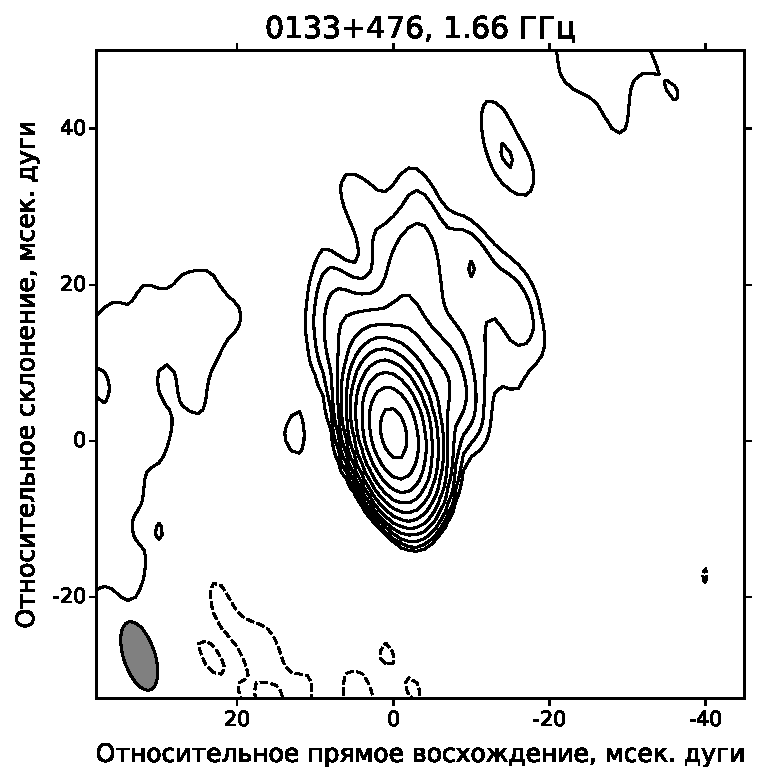
\includegraphics[width=0.3\textwidth]{0133+476_L.pdf}
  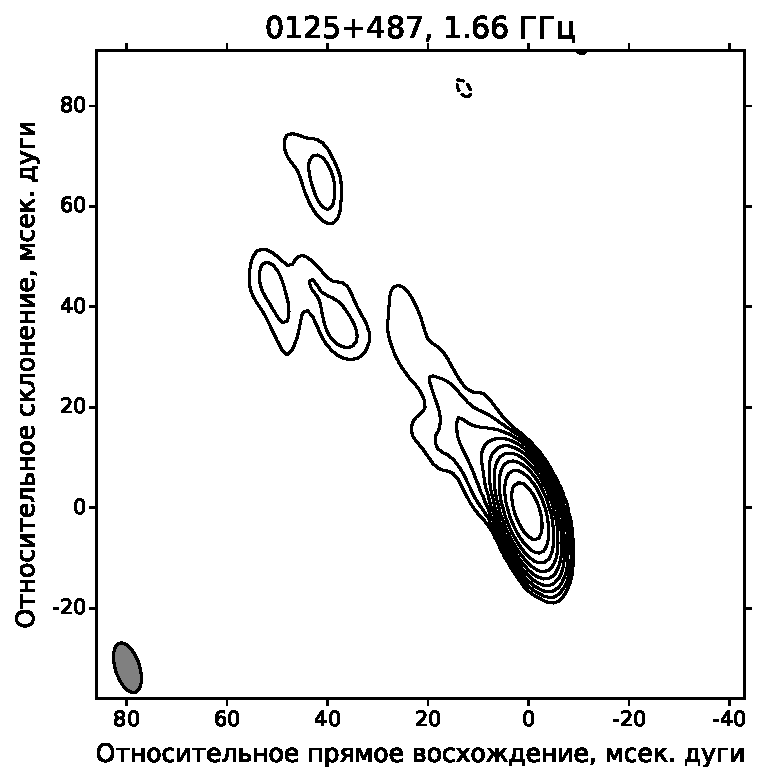
\includegraphics[width=0.3\textwidth]{0125+487_L.pdf}
  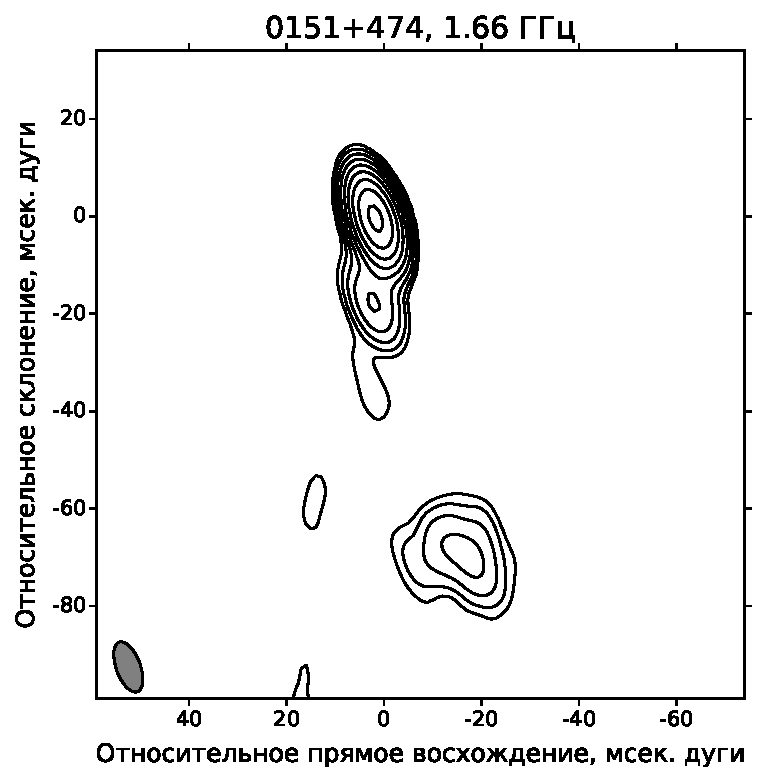
\includegraphics[width=0.3\textwidth]{0151+474_L.pdf}


  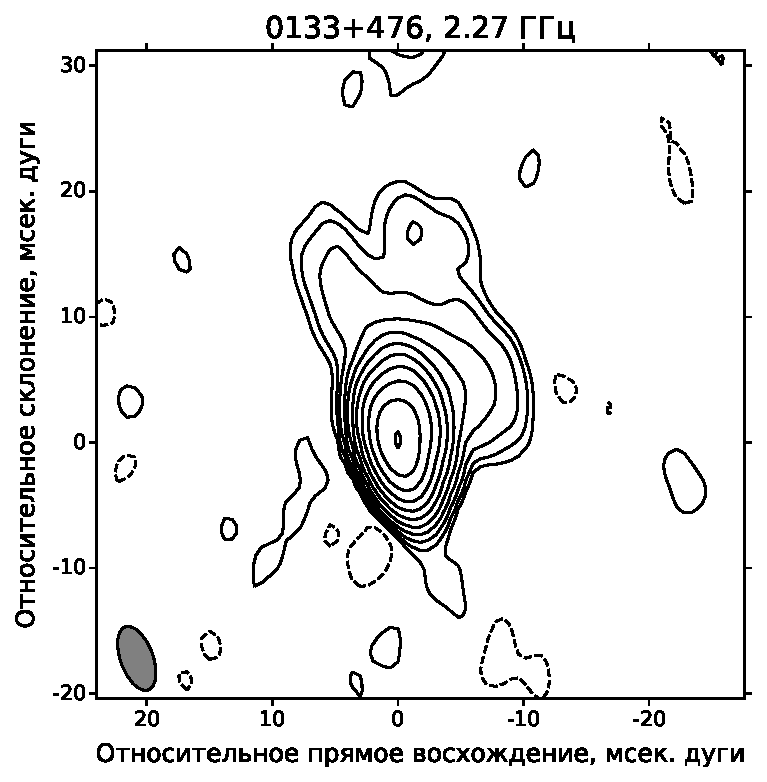
\includegraphics[width=0.3\textwidth]{0133+476_S.pdf}
  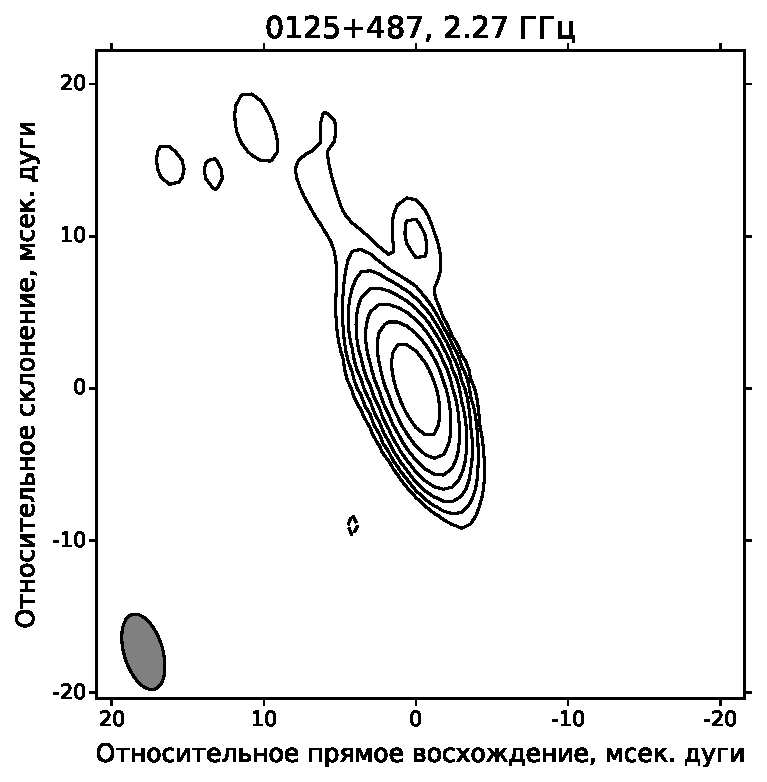
\includegraphics[width=0.3\textwidth]{0125+487_S.pdf}
  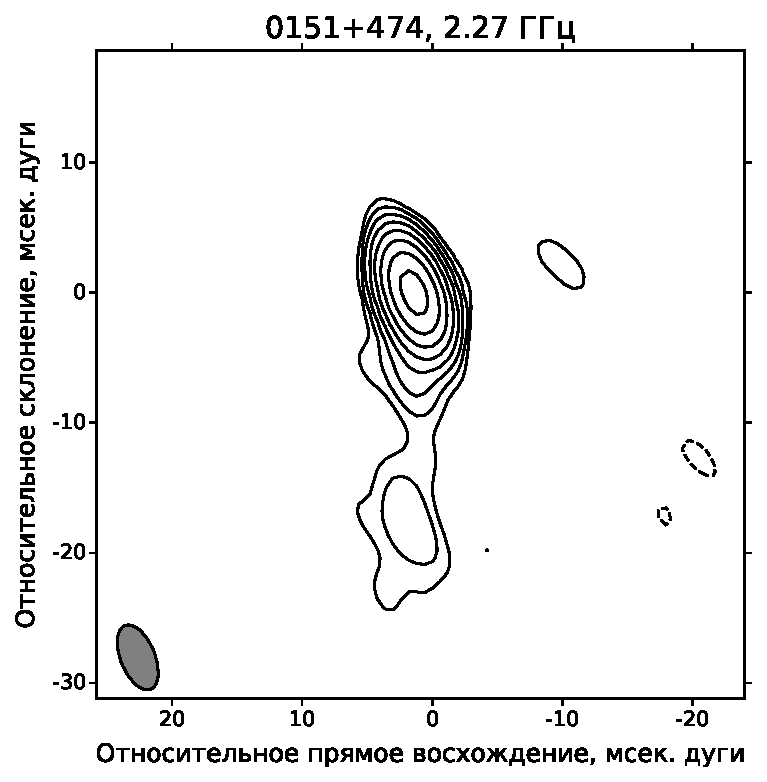
\includegraphics[width=0.3\textwidth]{0151+474_S.pdf}


  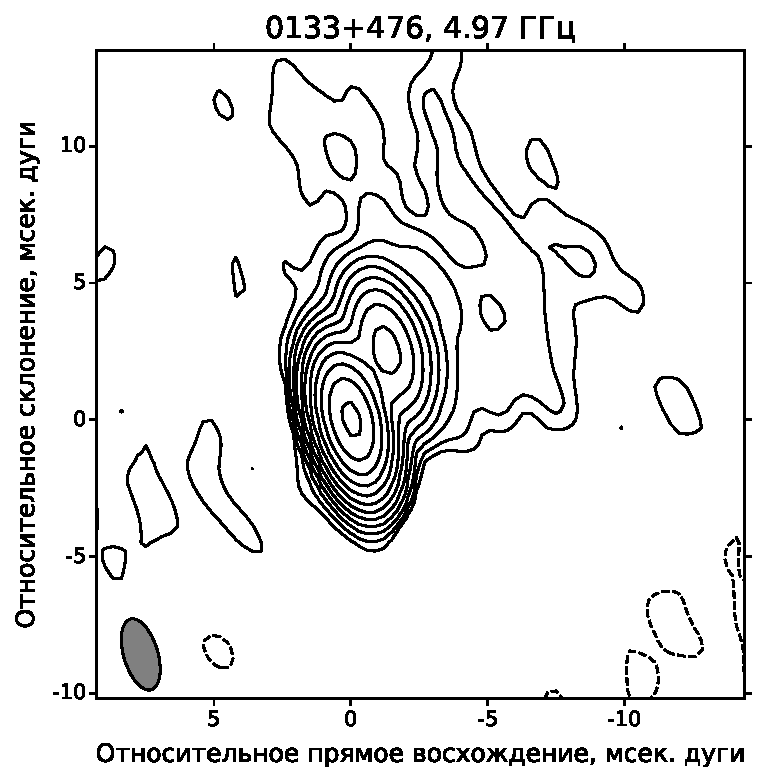
\includegraphics[width=0.3\textwidth]{0133+476_C.pdf}
  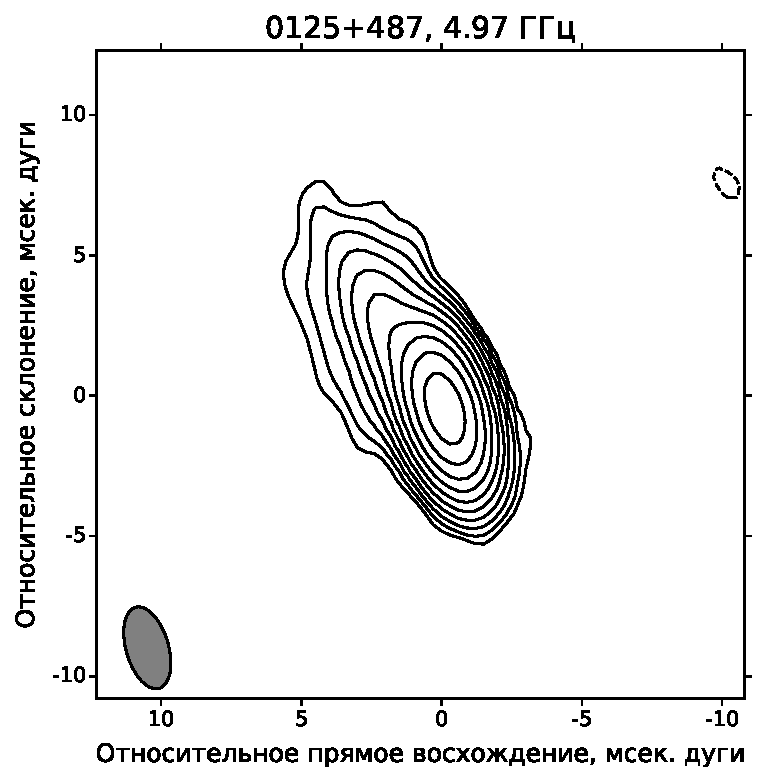
\includegraphics[width=0.3\textwidth]{0125+487_C.pdf}
  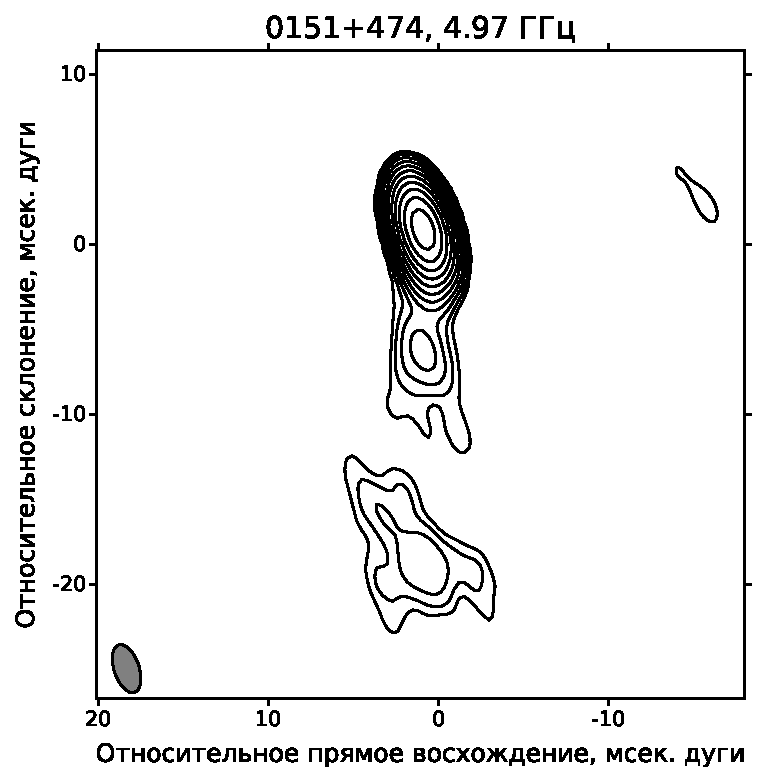
\includegraphics[width=0.3\textwidth]{0151+474_C.pdf}


  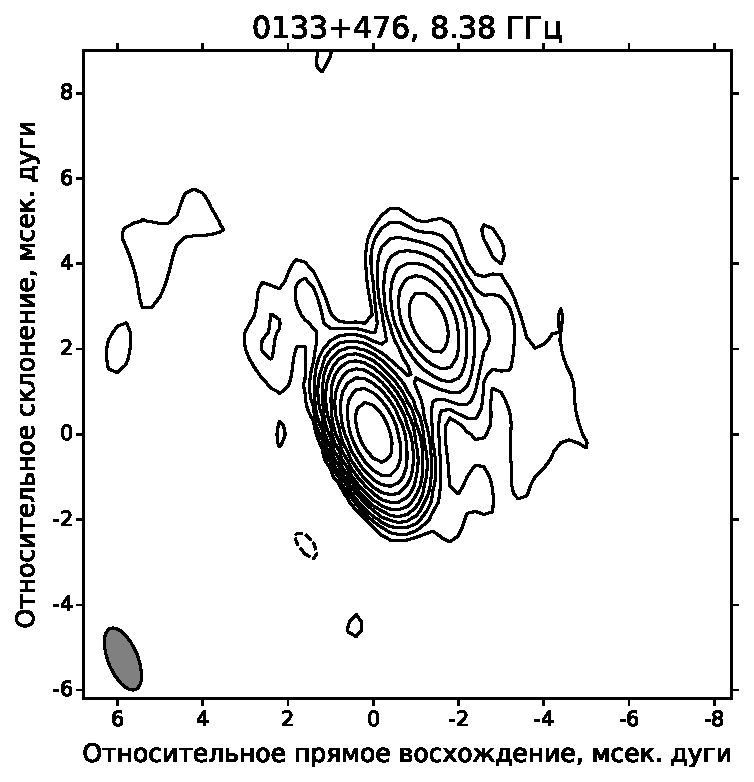
\includegraphics[width=0.3\textwidth]{0133+476_X.pdf}
  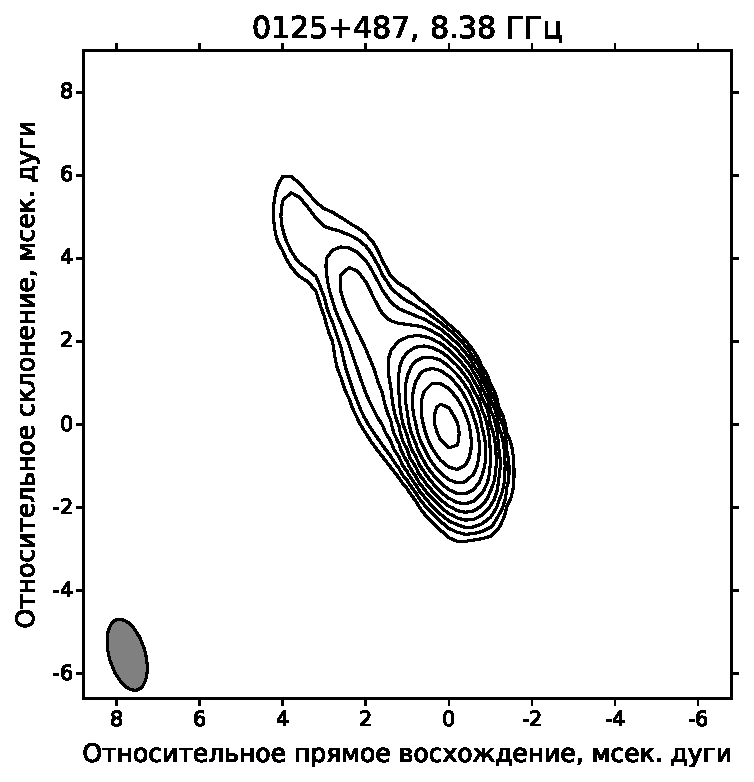
\includegraphics[width=0.3\textwidth]{0125+487_X.pdf}
  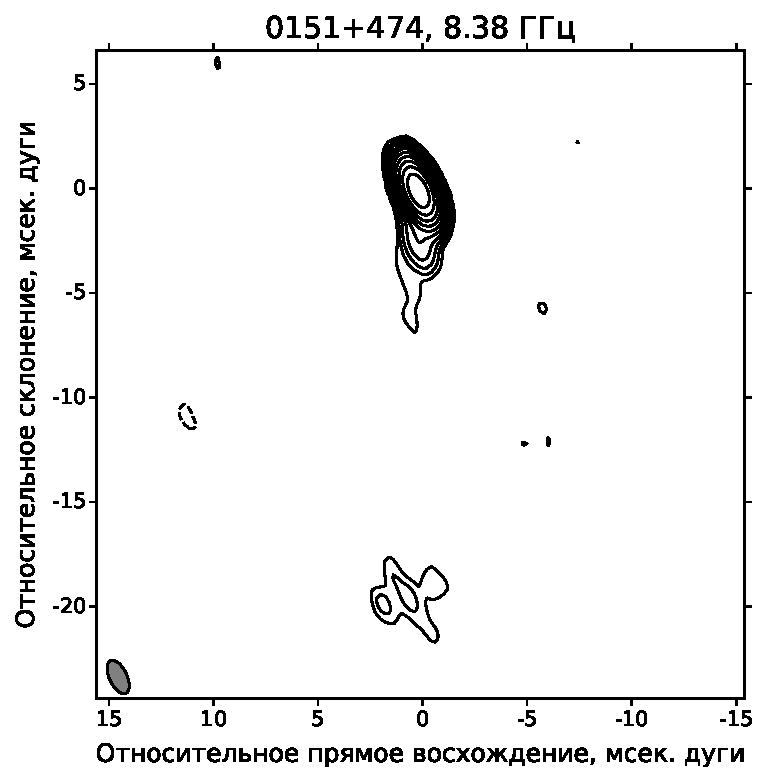
\includegraphics[width=0.3\textwidth]{0151+474_X.pdf}

  \caption{Карты полной интенсивности всех наблюдаемых источников с натуральным взвешиванием данных.
Первый контур проведен по уровню 3 RMS остаточного шума.}
  \label{fig:maps}
\end{figure}

\addtocounter{figure}{-1}
\begin{figure}
  \centering

  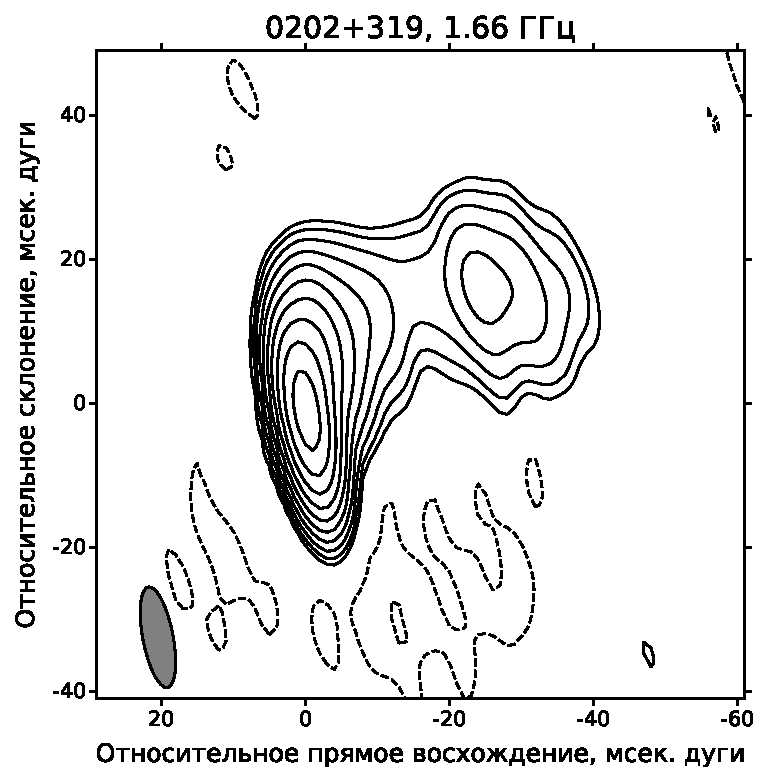
\includegraphics[width=0.3\textwidth]{0202+319_L.pdf}
  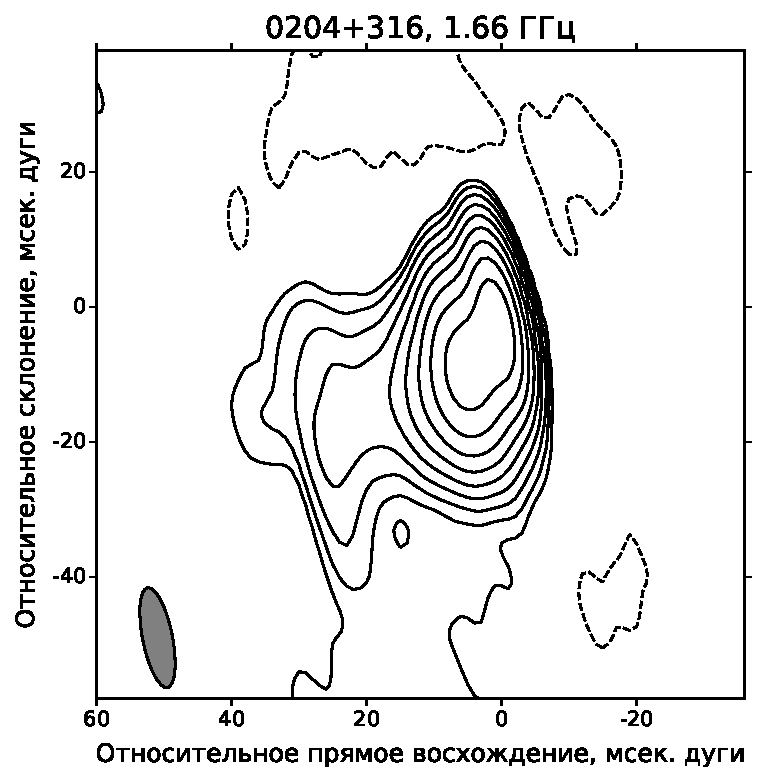
\includegraphics[width=0.3\textwidth]{0204+316_L.pdf}
  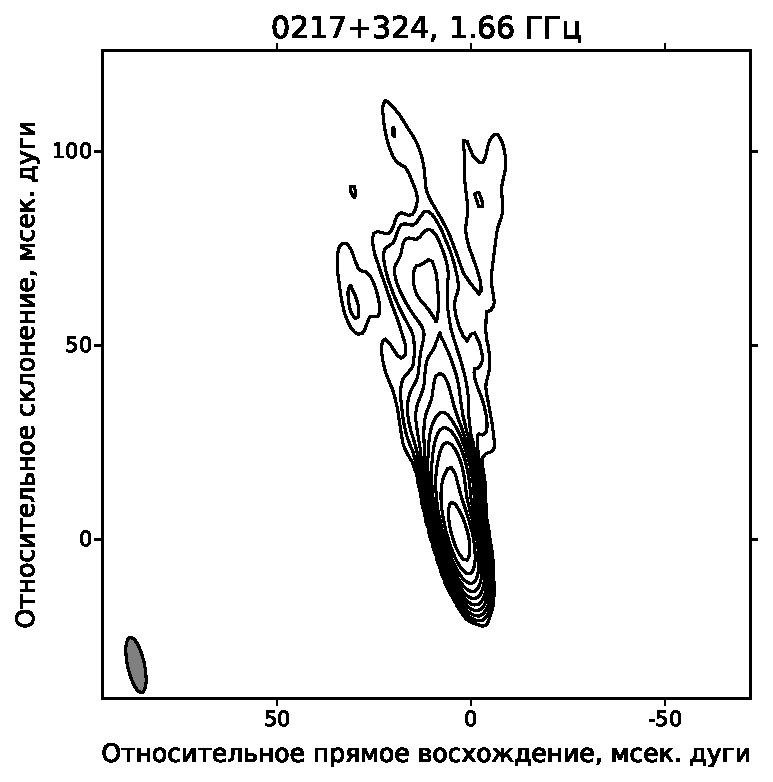
\includegraphics[width=0.3\textwidth]{0217+324_L.pdf}


  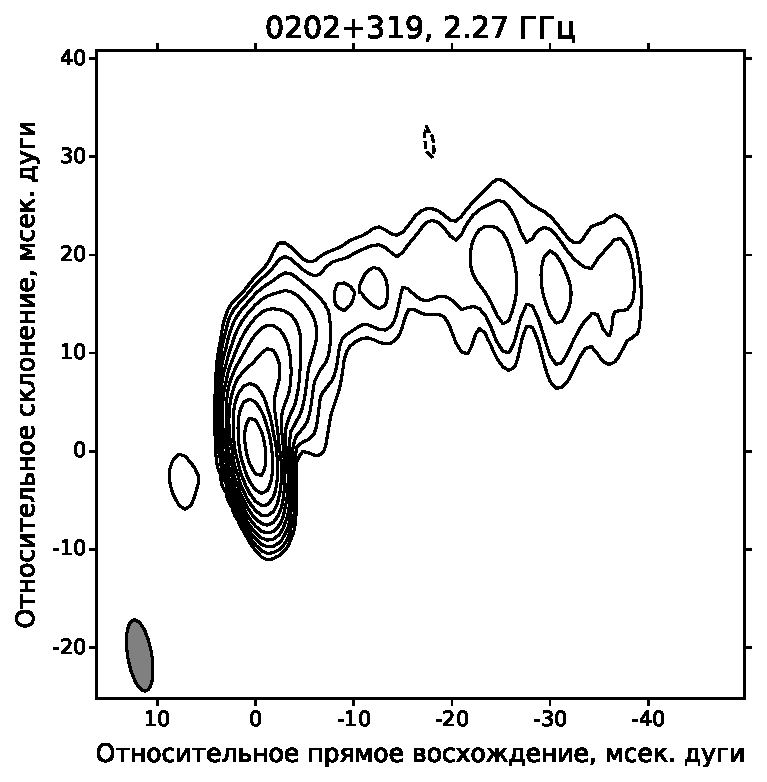
\includegraphics[width=0.3\textwidth]{0202+319_S.pdf}
  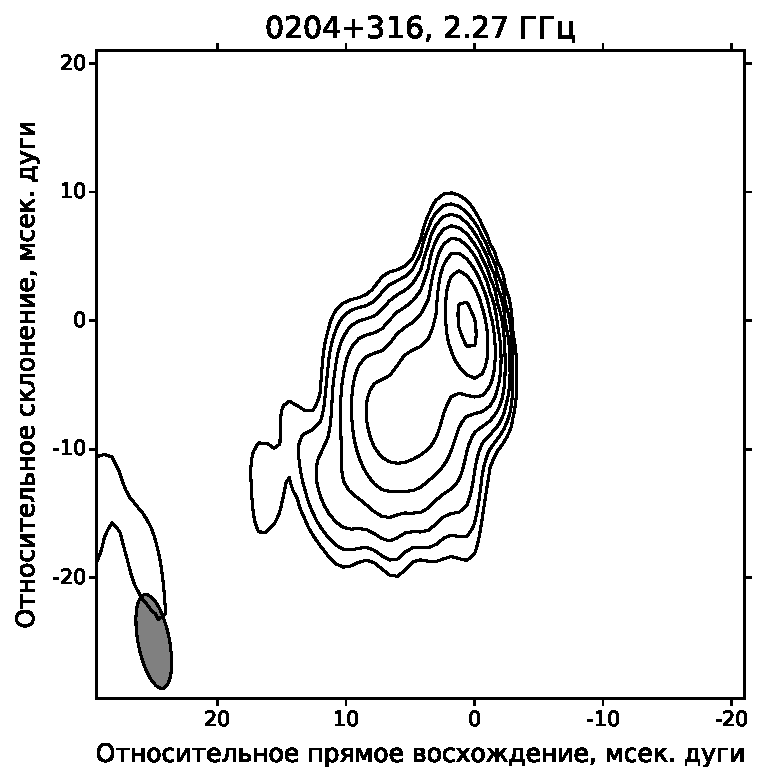
\includegraphics[width=0.3\textwidth]{0204+316_S.pdf}
  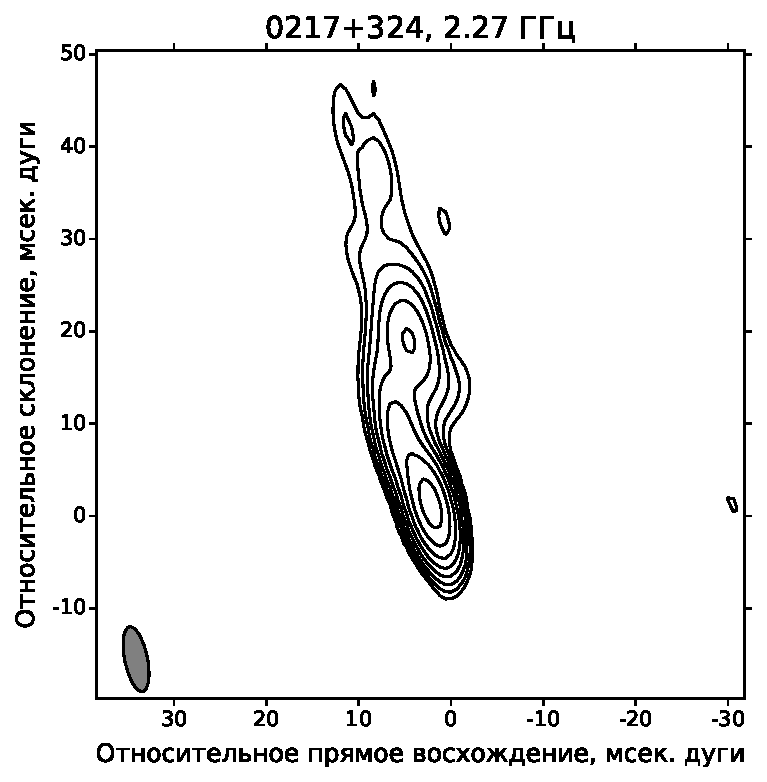
\includegraphics[width=0.3\textwidth]{0217+324_S.pdf}


  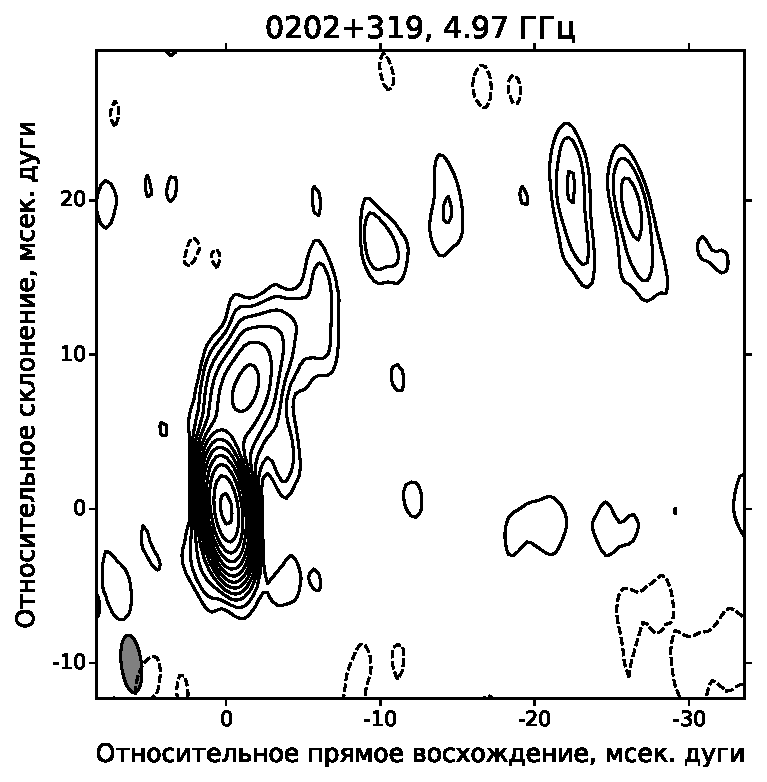
\includegraphics[width=0.3\textwidth]{0202+319_C.pdf}
  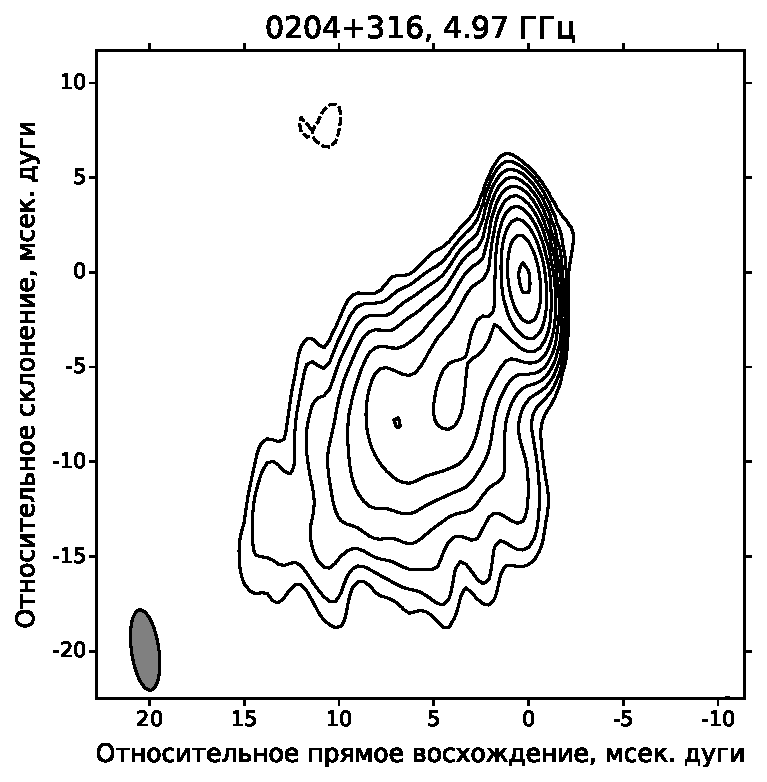
\includegraphics[width=0.3\textwidth]{0204+316_C.pdf}
  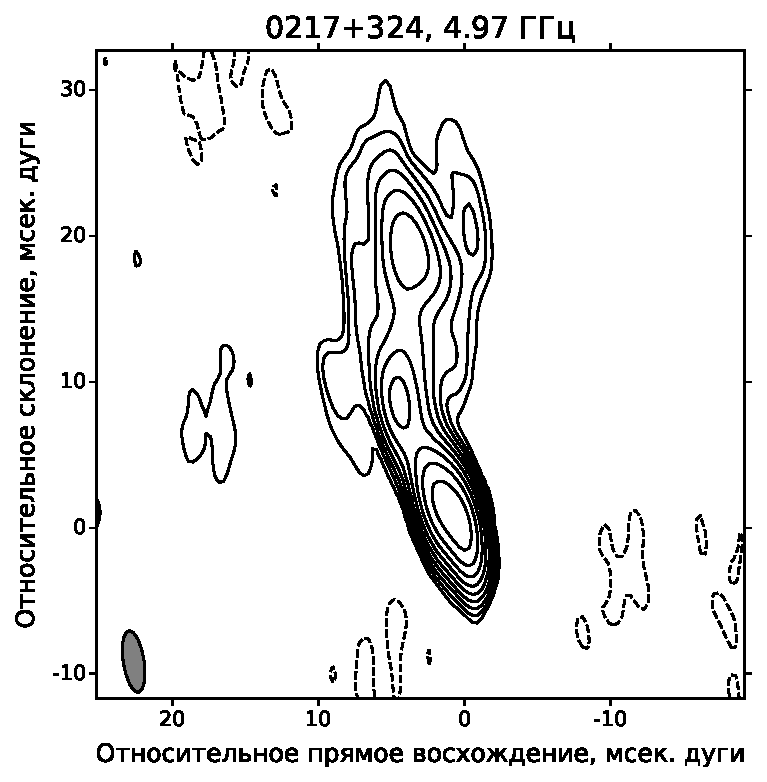
\includegraphics[width=0.3\textwidth]{0217+324_C.pdf}


  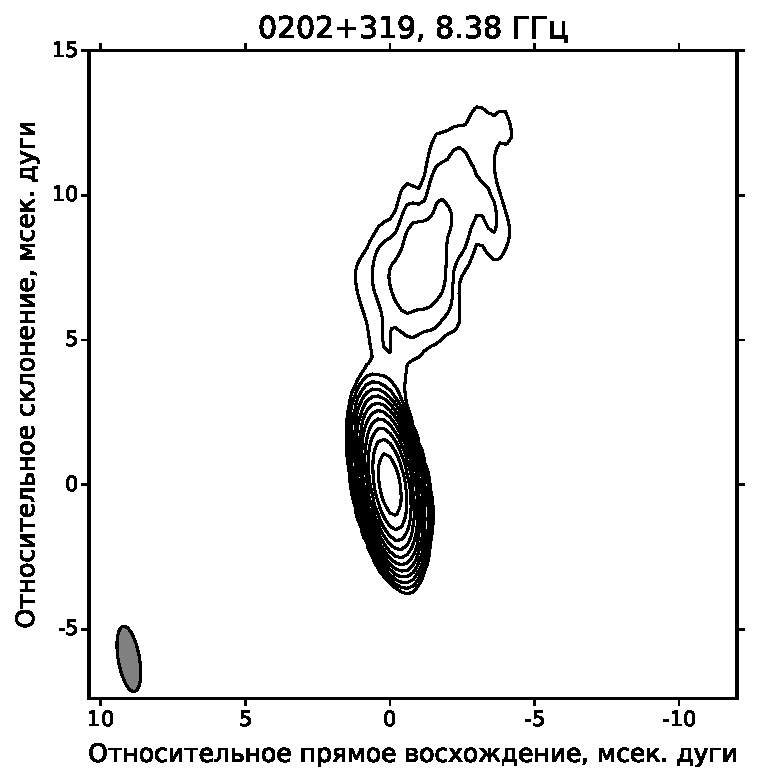
\includegraphics[width=0.3\textwidth]{0202+319_X.pdf}
  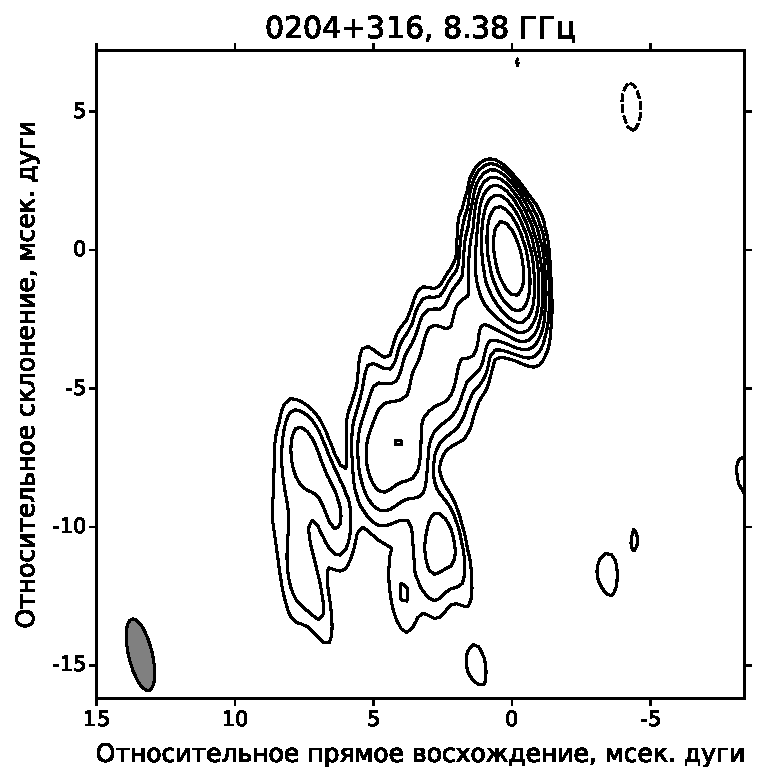
\includegraphics[width=0.3\textwidth]{0204+316_X.pdf}
  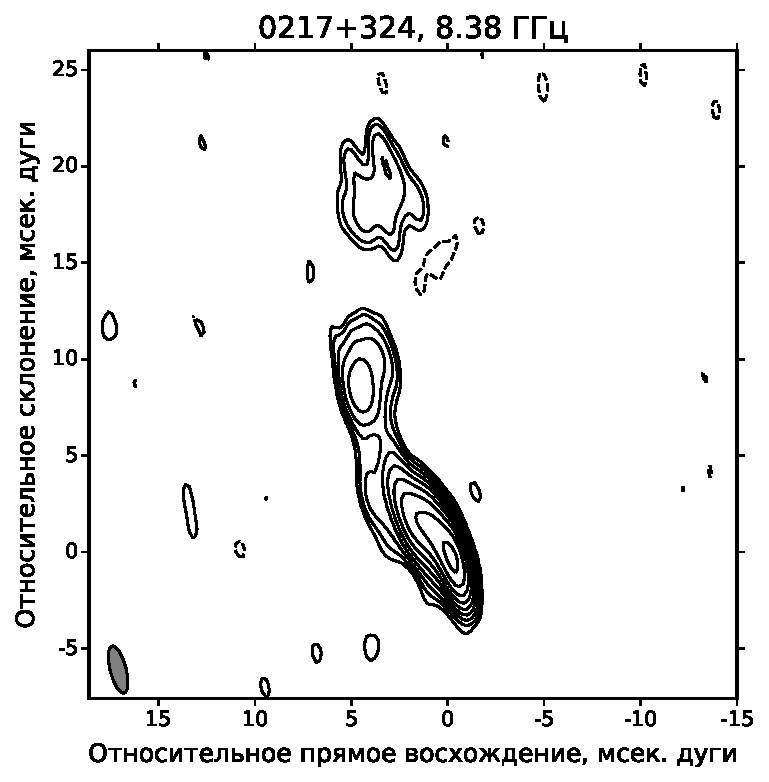
\includegraphics[width=0.3\textwidth]{0217+324_X.pdf}

  \caption{продолжение...}
\end{figure}

\addtocounter{figure}{-1}
\begin{figure}
  \centering

  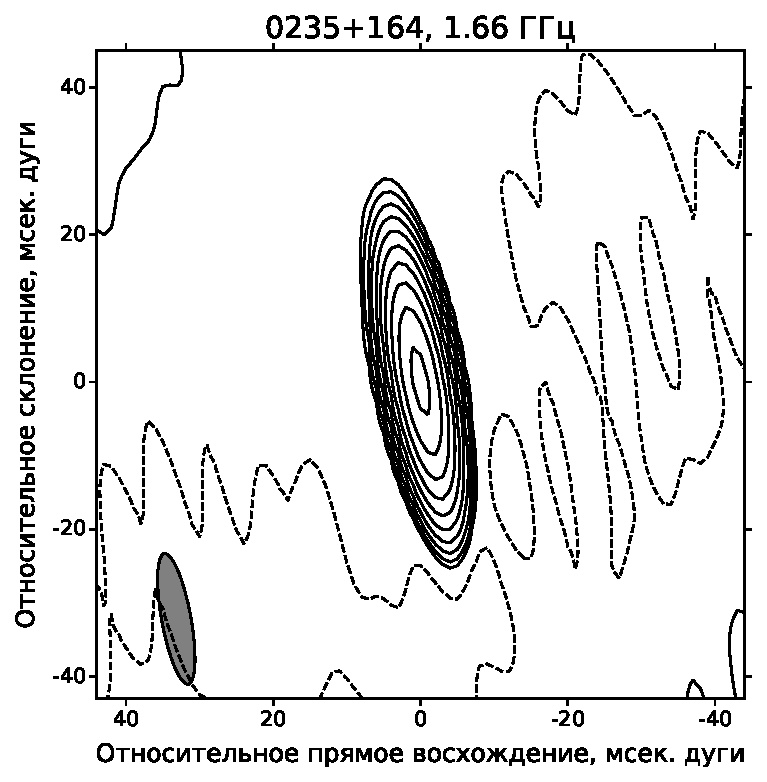
\includegraphics[width=0.3\textwidth]{0235+164_L.pdf}
  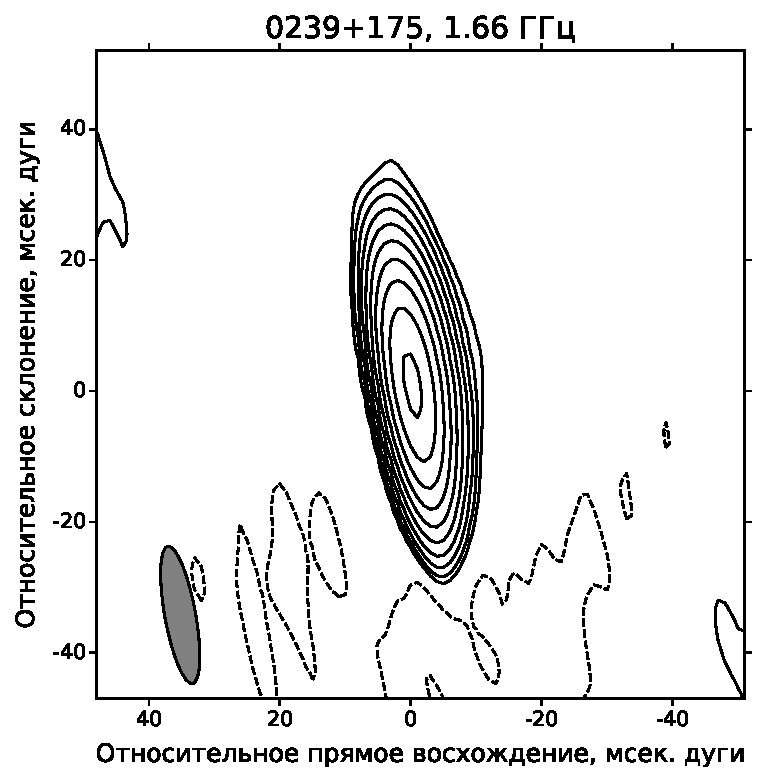
\includegraphics[width=0.3\textwidth]{0239+175_L.pdf}
  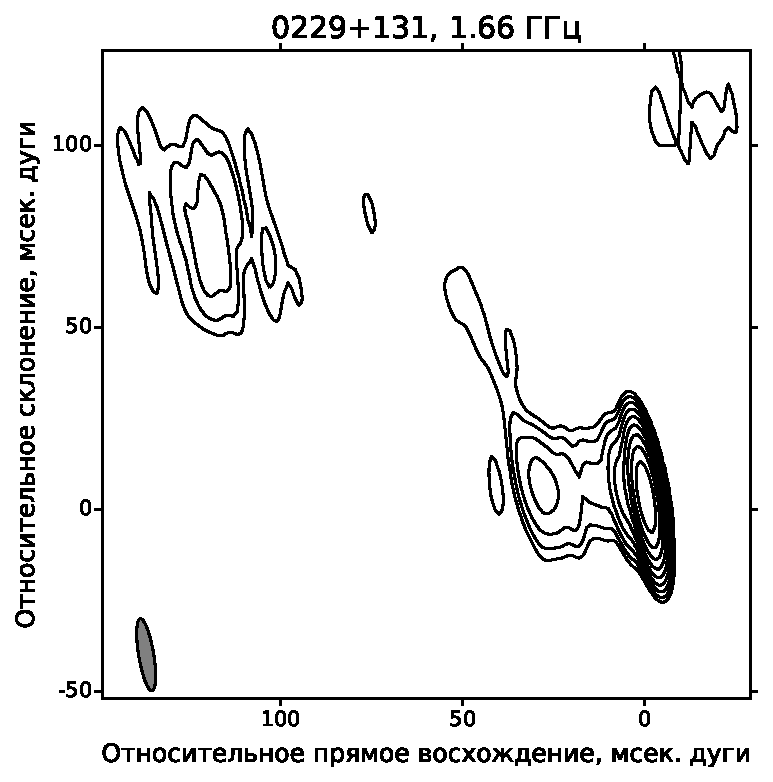
\includegraphics[width=0.3\textwidth]{0229+131_L.pdf}


  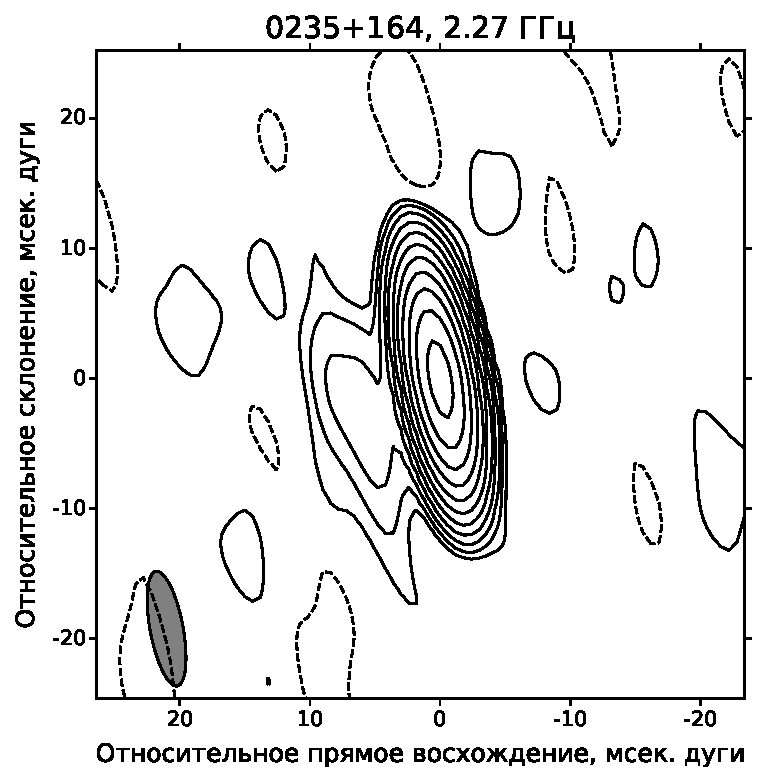
\includegraphics[width=0.3\textwidth]{0235+164_S.pdf}
  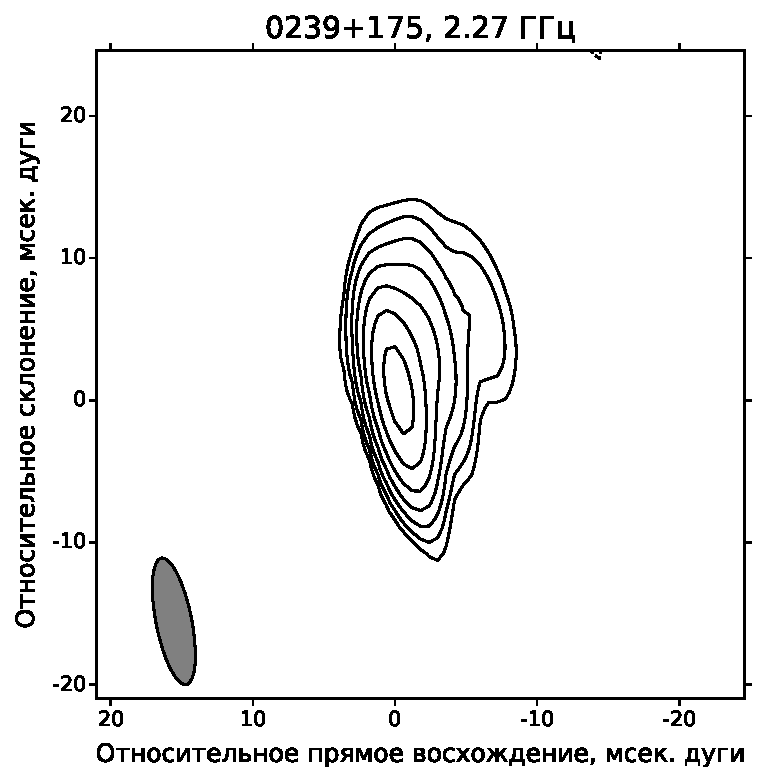
\includegraphics[width=0.3\textwidth]{0239+175_S.pdf}
  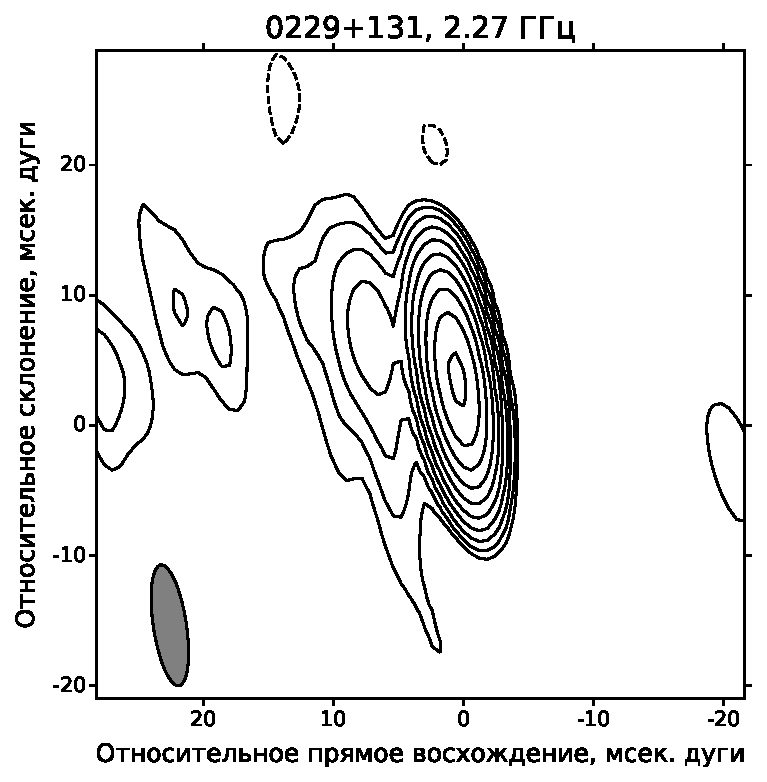
\includegraphics[width=0.3\textwidth]{0229+131_S.pdf}


  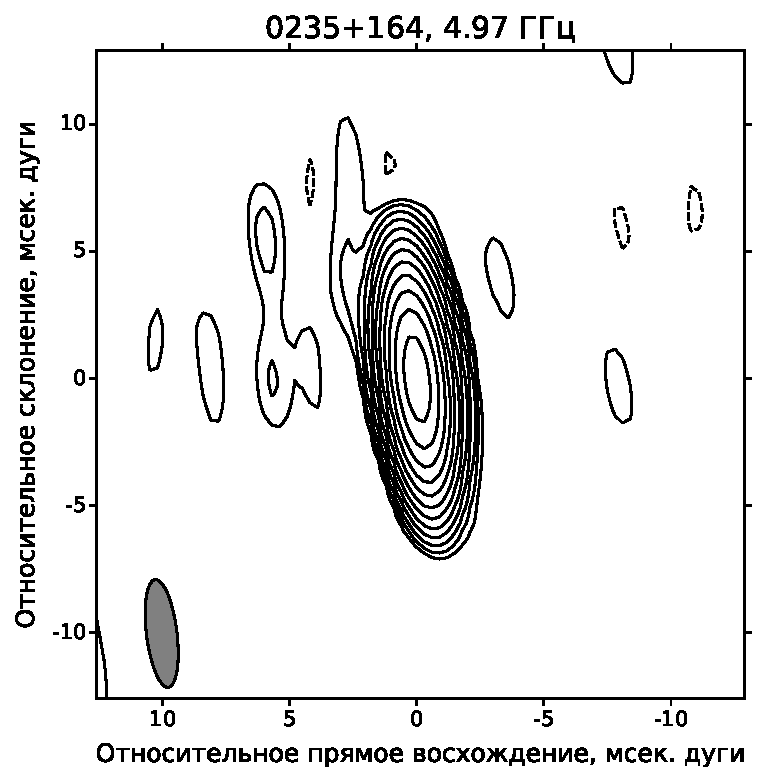
\includegraphics[width=0.3\textwidth]{0235+164_C.pdf}
  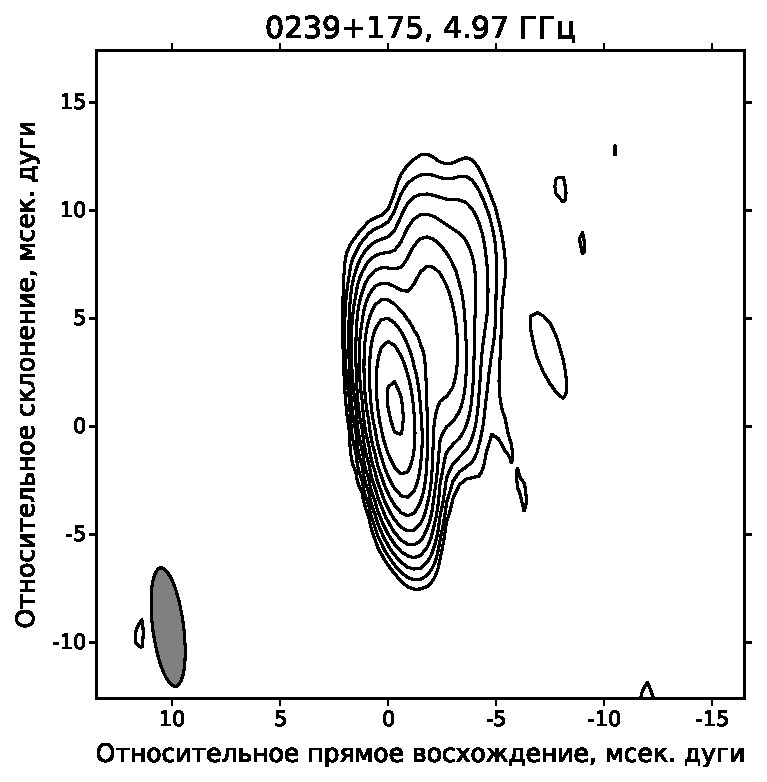
\includegraphics[width=0.3\textwidth]{0239+175_C.pdf}
  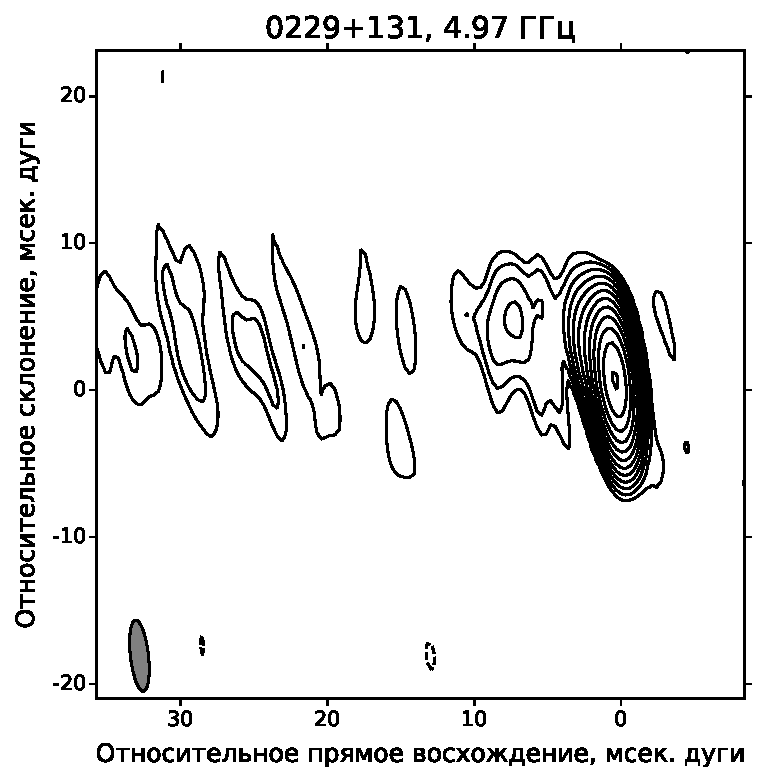
\includegraphics[width=0.3\textwidth]{0229+131_C.pdf}


  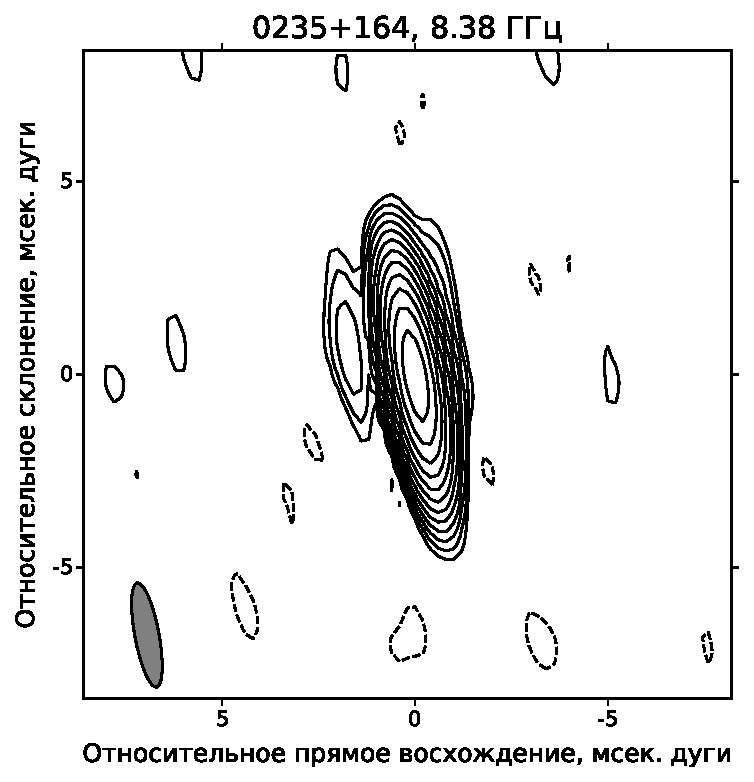
\includegraphics[width=0.3\textwidth]{0235+164_X.pdf}
  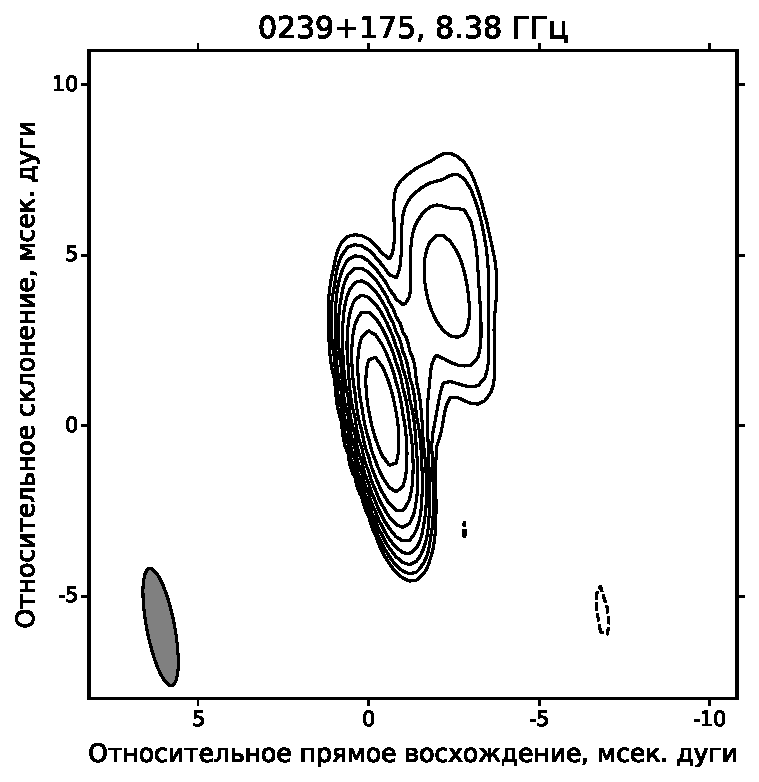
\includegraphics[width=0.3\textwidth]{0239+175_X.pdf}
  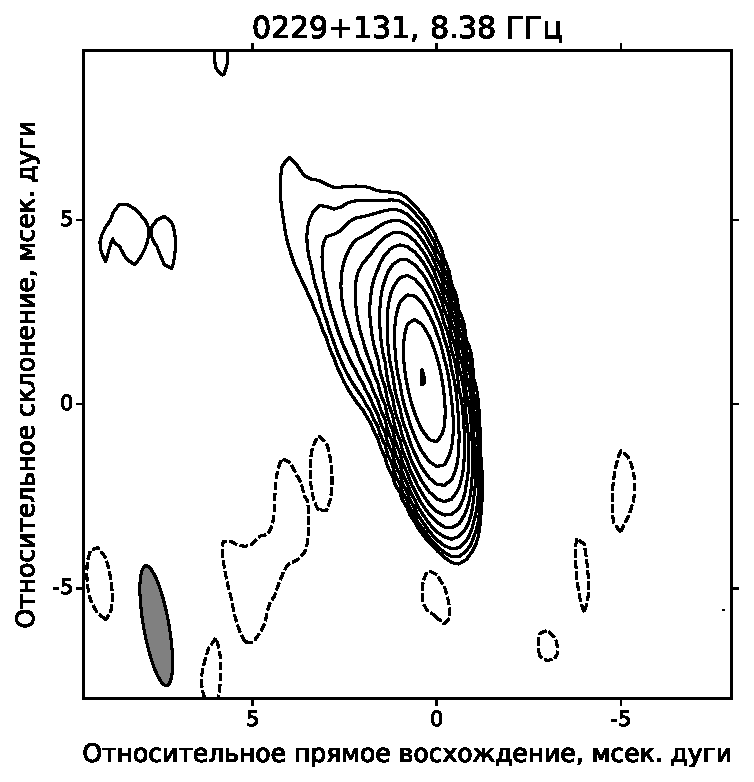
\includegraphics[width=0.3\textwidth]{0229+131_X.pdf}

  \caption{продолжение...}
\end{figure}

\addtocounter{figure}{-1}
\begin{figure}
  \centering

  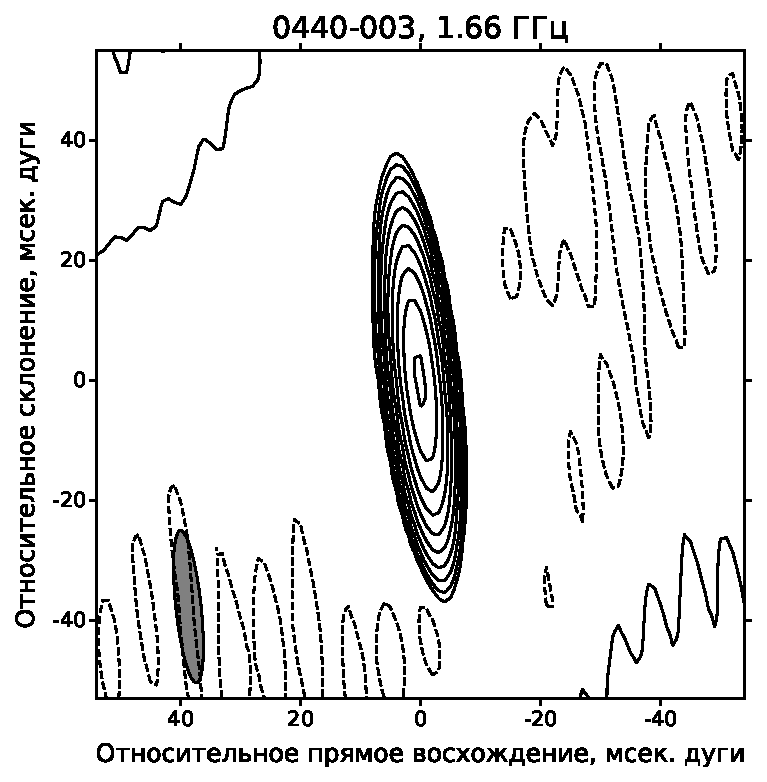
\includegraphics[width=0.3\textwidth]{0440-003_L.pdf}
  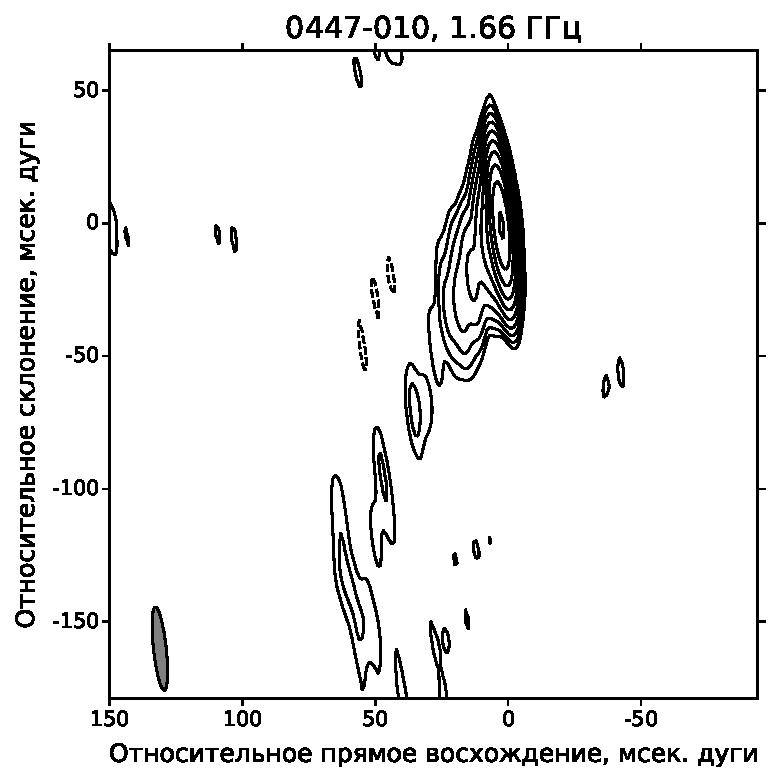
\includegraphics[width=0.3\textwidth]{0447-010_L.pdf}
  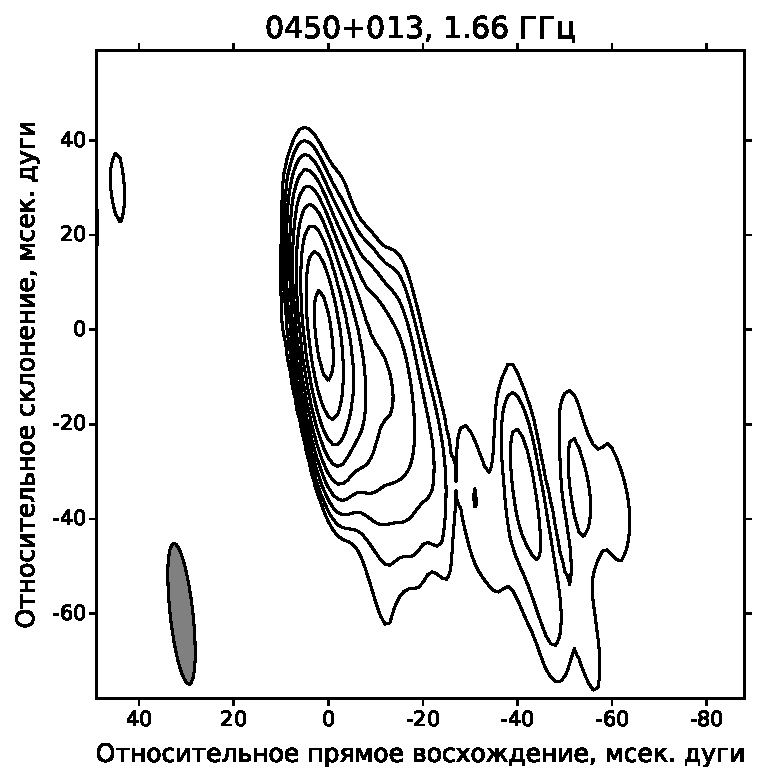
\includegraphics[width=0.3\textwidth]{0450+013_L.pdf}


  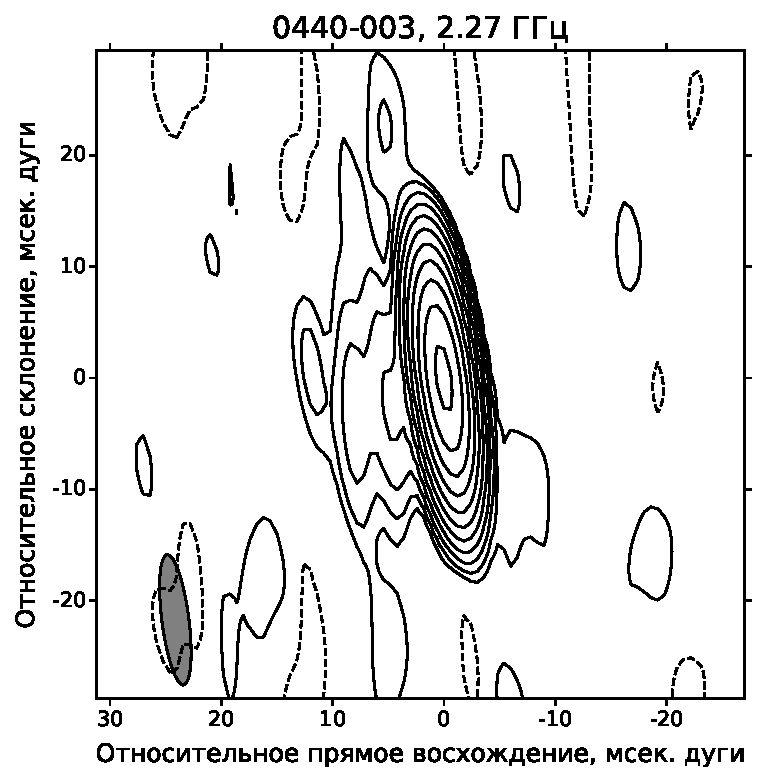
\includegraphics[width=0.3\textwidth]{0440-003_S.pdf}
  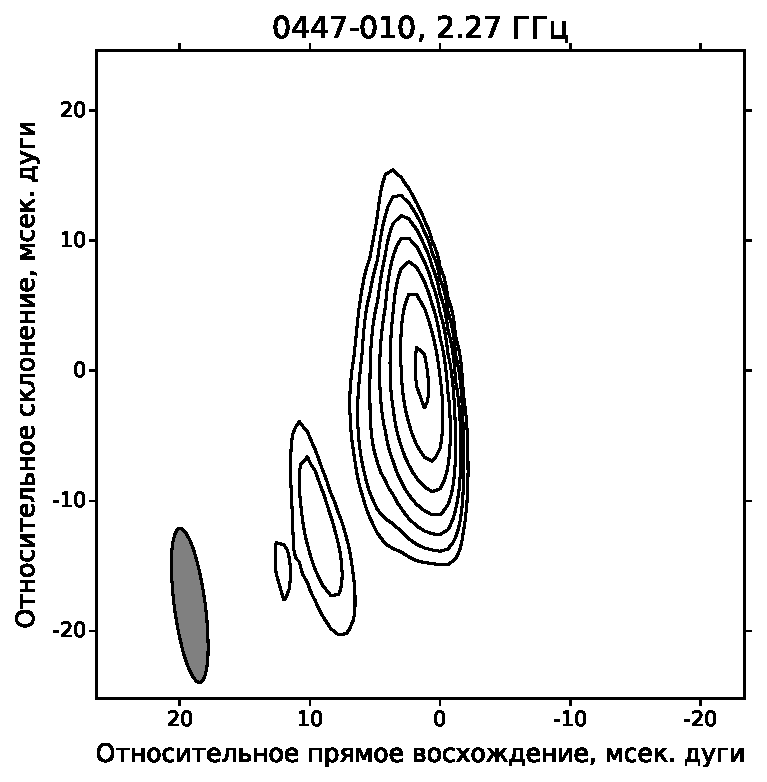
\includegraphics[width=0.3\textwidth]{0447-010_S.pdf}
  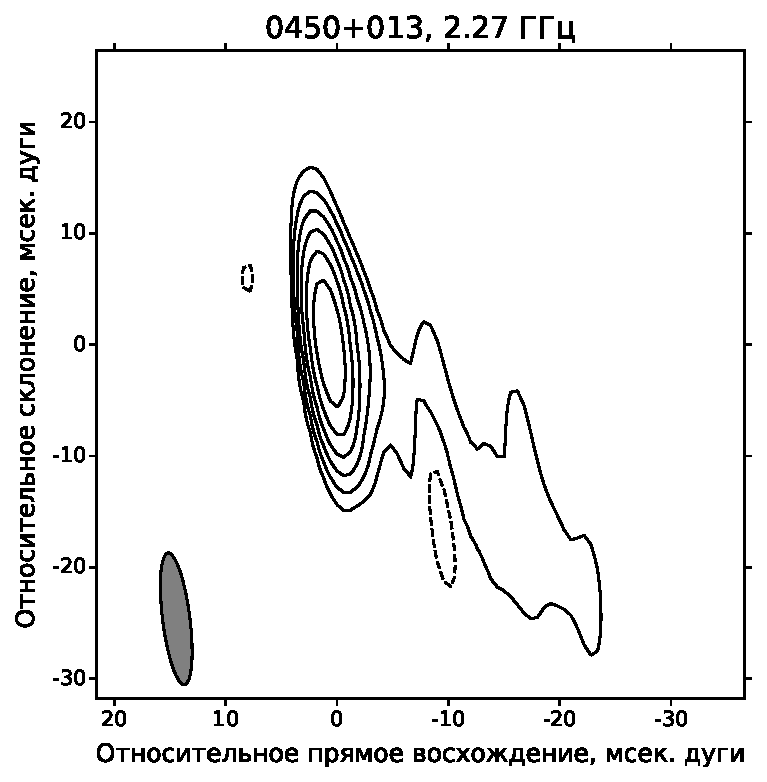
\includegraphics[width=0.3\textwidth]{0450+013_S.pdf}


  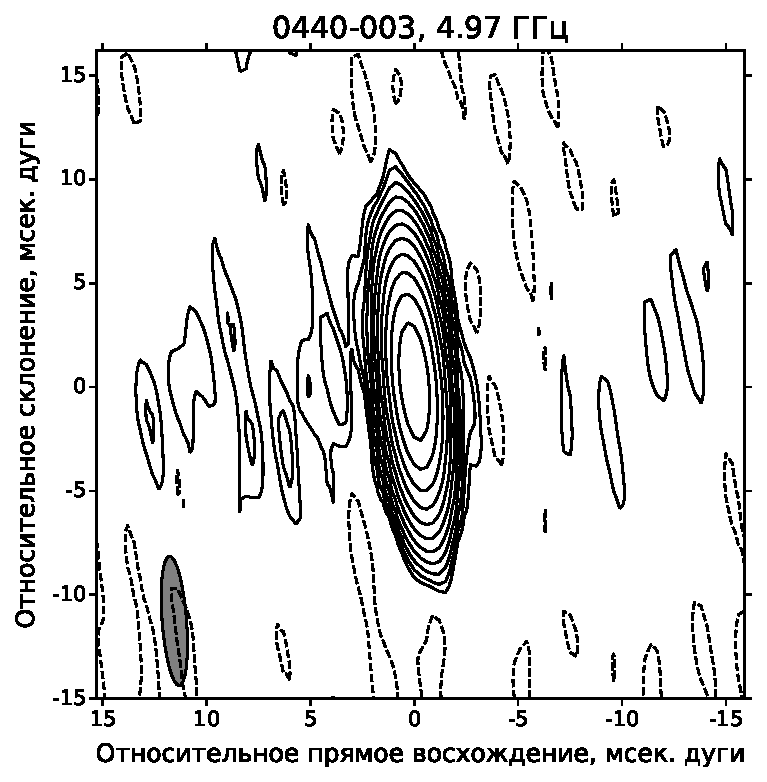
\includegraphics[width=0.3\textwidth]{0440-003_C.pdf}
  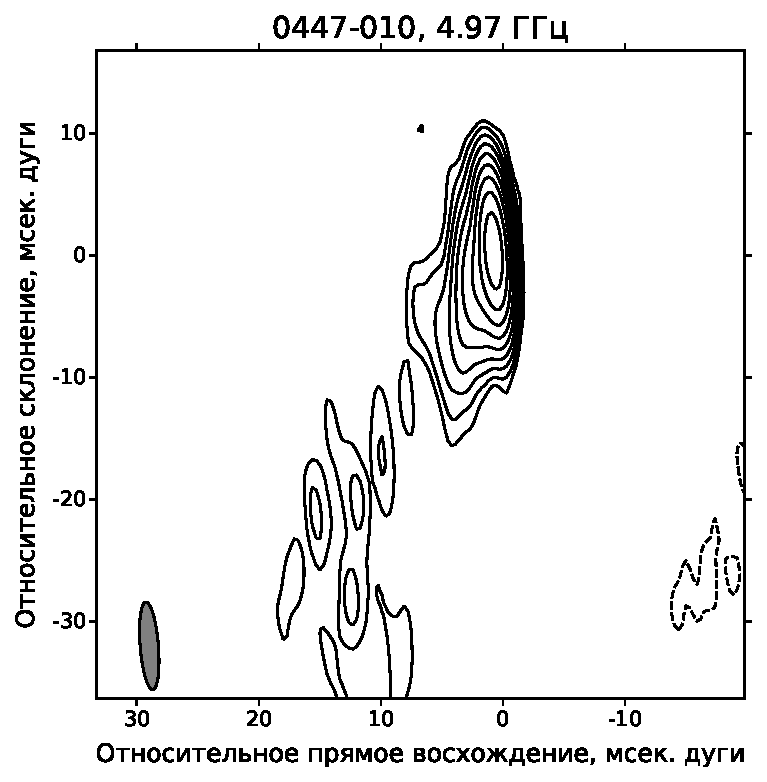
\includegraphics[width=0.3\textwidth]{0447-010_C.pdf}
  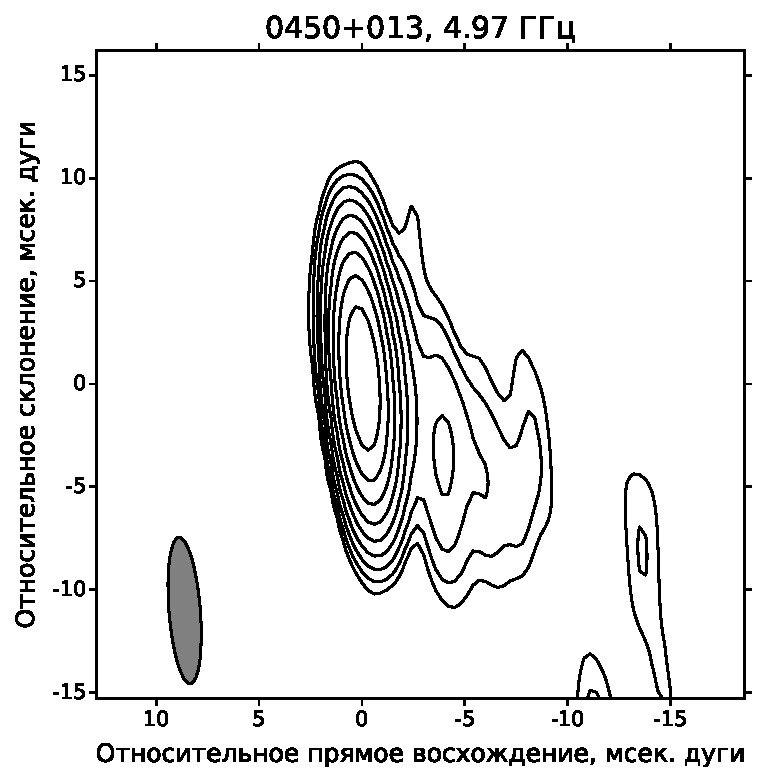
\includegraphics[width=0.3\textwidth]{0450+013_C.pdf}


  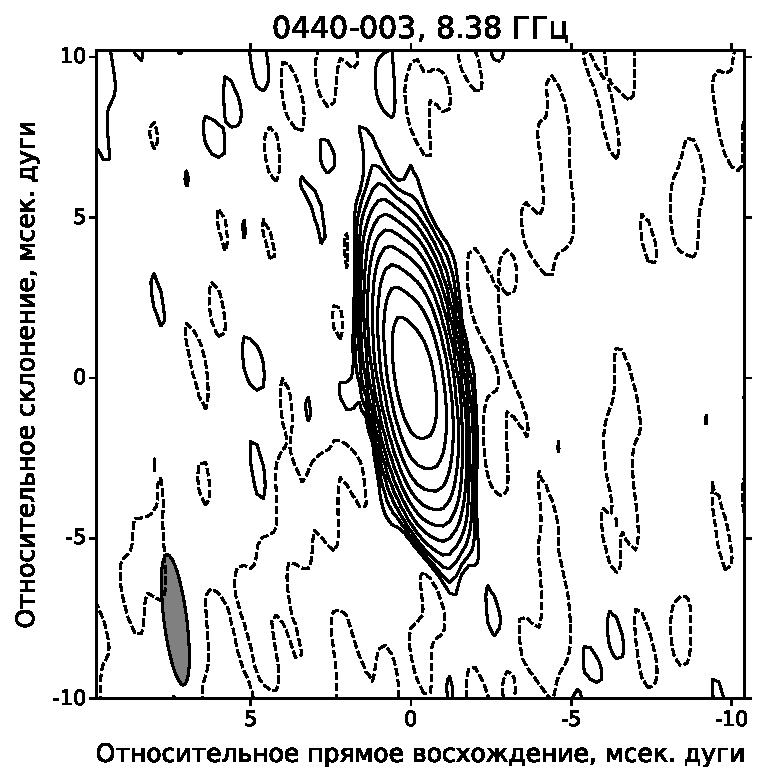
\includegraphics[width=0.3\textwidth]{0440-003_X.pdf}
  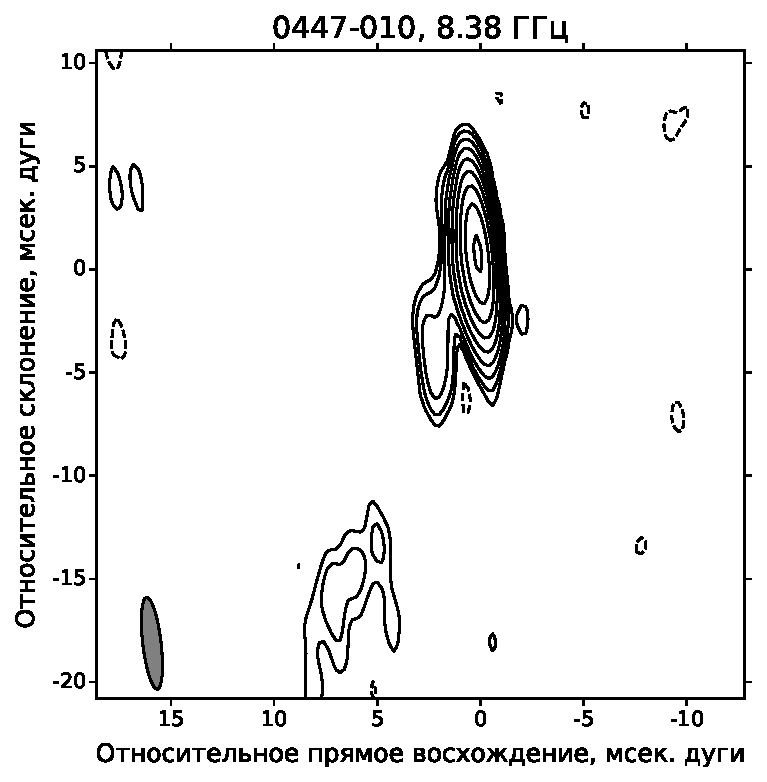
\includegraphics[width=0.3\textwidth]{0447-010_X.pdf}
  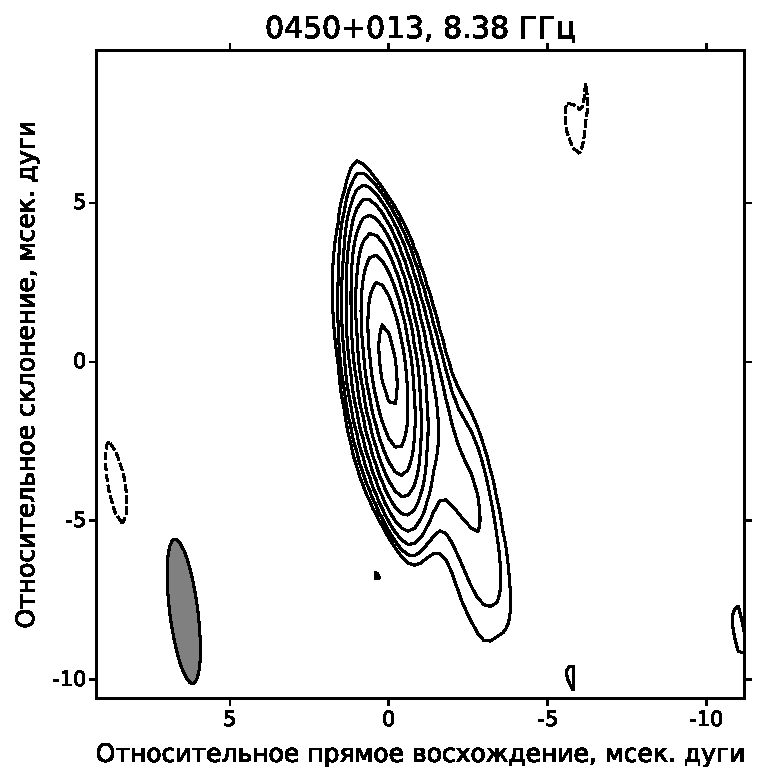
\includegraphics[width=0.3\textwidth]{0450+013_X.pdf}

  \caption{продолжение...}
\end{figure}

\addtocounter{figure}{-1}
\begin{figure}
  \centering

  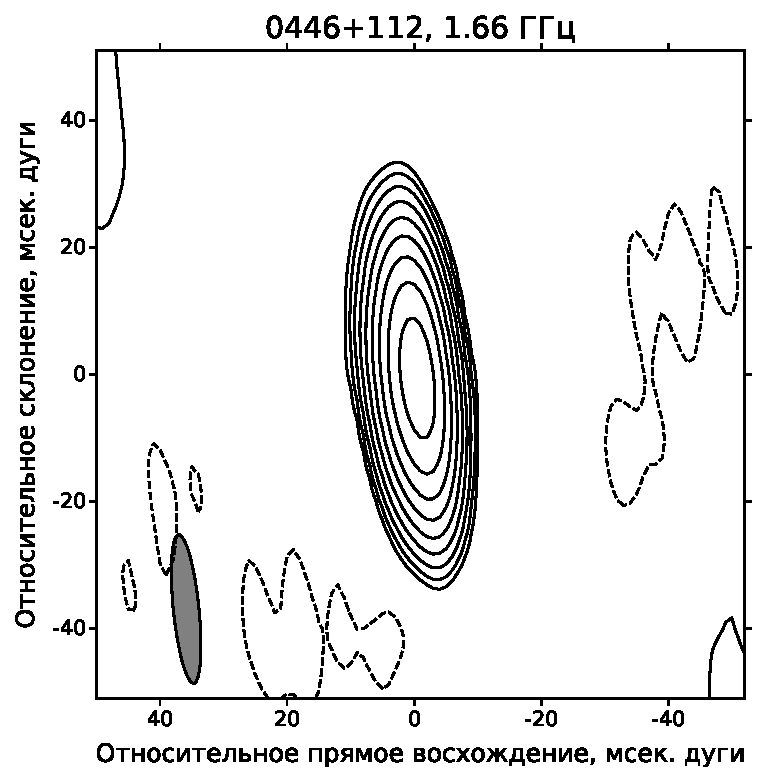
\includegraphics[width=0.3\textwidth]{0446+112_L.pdf}
  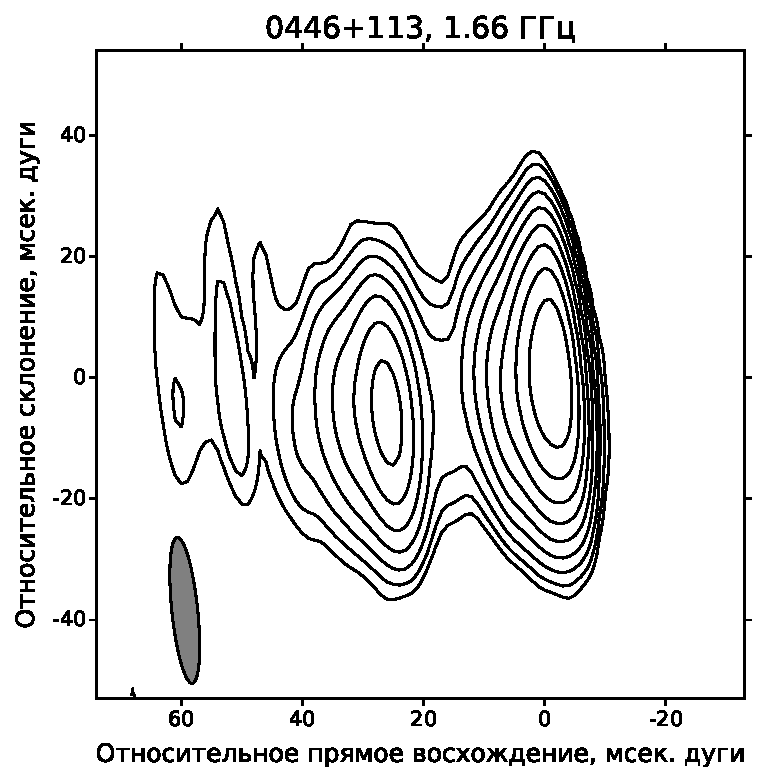
\includegraphics[width=0.3\textwidth]{0446+113_L.pdf}
  \includegraphics[width=0.3\textwidth]{0445+097_L.pdf}


  \includegraphics[width=0.3\textwidth]{0446+112_S.pdf}
  \includegraphics[width=0.3\textwidth]{0446+113_S.pdf}
  \includegraphics[width=0.3\textwidth]{0445+097_S.pdf}


  \includegraphics[width=0.3\textwidth]{0446+112_C.pdf}
  \includegraphics[width=0.3\textwidth]{0446+113_C.pdf}
  \includegraphics[width=0.3\textwidth]{0445+097_C.pdf}


  \includegraphics[width=0.3\textwidth]{0446+112_X.pdf}
  \includegraphics[width=0.3\textwidth]{0446+113_X.pdf}
  \includegraphics[width=0.3\textwidth]{0445+097_X.pdf}

  \caption{продолжение...}
\end{figure}

\addtocounter{figure}{-1}
\begin{figure}
  \centering

  \includegraphics[width=0.3\textwidth]{1749+096_L.pdf}
  \includegraphics[width=0.3\textwidth]{1745+085_L.pdf}
  \includegraphics[width=0.3\textwidth]{1749+062_L.pdf}


  \includegraphics[width=0.3\textwidth]{1749+096_S.pdf}
  \includegraphics[width=0.3\textwidth]{1745+085_S.pdf}
  \includegraphics[width=0.3\textwidth]{1749+062_S.pdf}


  \includegraphics[width=0.3\textwidth]{1749+096_C.pdf}
  \includegraphics[width=0.3\textwidth]{1745+085_C.pdf}
  \includegraphics[width=0.3\textwidth]{1749+062_C.pdf}


  \includegraphics[width=0.3\textwidth]{1749+096_X.pdf}
  \includegraphics[width=0.3\textwidth]{1745+085_X.pdf}
  \includegraphics[width=0.3\textwidth]{1749+062_X.pdf}

  \caption{продолжение...}
\end{figure}

\addtocounter{figure}{-1}
\begin{figure}
  \centering

  \includegraphics[width=0.3\textwidth]{2136+141_L.pdf}
  \includegraphics[width=0.3\textwidth]{2137+130_L.pdf}
  \includegraphics[width=0.3\textwidth]{2141+175_L.pdf}


  \includegraphics[width=0.3\textwidth]{2136+141_S.pdf}
  \includegraphics[width=0.3\textwidth]{2137+130_S.pdf}
  \includegraphics[width=0.3\textwidth]{2141+175_S.pdf}


  \includegraphics[width=0.3\textwidth]{2136+141_C.pdf}
  \includegraphics[width=0.3\textwidth]{2137+130_C.pdf}
  \includegraphics[width=0.3\textwidth]{2141+175_C.pdf}


  \includegraphics[width=0.3\textwidth]{2136+141_X.pdf}
  \includegraphics[width=0.3\textwidth]{2137+130_X.pdf}
  \includegraphics[width=0.3\textwidth]{2141+175_X.pdf}

  \caption{продолжение...}
\end{figure}

\addtocounter{figure}{-1}
\begin{figure}
  \centering

  \includegraphics[width=0.3\textwidth]{2145+067_L.pdf}
  \includegraphics[width=0.3\textwidth]{2149+056_L.pdf}
  \includegraphics[width=0.3\textwidth]{2144+092_L.pdf}


  \includegraphics[width=0.3\textwidth]{2145+067_S.pdf}
  \includegraphics[width=0.3\textwidth]{2149+056_S.pdf}
  \includegraphics[width=0.3\textwidth]{2144+092_S.pdf}


  \includegraphics[width=0.3\textwidth]{2145+067_C.pdf}
  \includegraphics[width=0.3\textwidth]{2149+056_C.pdf}
  \includegraphics[width=0.3\textwidth]{2144+092_C.pdf}


  \includegraphics[width=0.3\textwidth]{2145+067_X.pdf}
  \includegraphics[width=0.3\textwidth]{2149+056_X.pdf}
  \includegraphics[width=0.3\textwidth]{2144+092_X.pdf}

  \caption{продолжение...}
\end{figure}


\begin{figure}
 \centering
% %  \setcaptionmargin{5mm}
%  \onelinecaptionstrue
 \includegraphics[width=0.6\textwidth]{uv_plot.png}
%  \captionstyle{normal}
 \caption{Покрытие UV-плоскости для источника 0133+476 на частоте 5~ГГц. Черными точками
обозначены проекции баз с телескопами сети ``Квазар-КВО'', серыми~--- остальные базы.}
 \label{fig:uv}
\end{figure}

\begin{figure}
 \centering
%  \setcaptionmargin{5mm}
 \includegraphics[width=0.5\textwidth]{rms_plot.pdf}
 \caption{Сравнение уровня остаточного шума изображений, восстановленных с использованием данных с
          телескопов сети ``Квазар-КВО'' и без них. Медианное значение шума составляет
          величину 0.28 и 0.36~мЯн/луч, соответственно.}
 \label{fig:map_rms}
\end{figure}

\begin{figure}
%  \setcaptionmargin{5mm}
 \includegraphics[width=0.9\textwidth]{rel_astrometry_errors.pdf}
 \caption{Уровень точности относительной астрометрии в диапазонах
          1.7 (L), 2.3 (S), 5.0 (C), 8.4 (X)~ГГц в зависимости от
          углового расстояния между источниками. Стрелками показаны
          угловые расстояния между источниками в триплетах.}
 \label{fig:astro_err}
\end{figure}

\begin{figure}
 \centering
%  \setcaptionmargin{5mm}
 % \onelinecaptionstrue
%  \onelinecaptionsfalse
 \includegraphics[width=0.9\textwidth]{freqdep/0}
 \includegraphics[width=0.9\textwidth]{freqdep/1}
 \includegraphics[width=0.9\textwidth]{freqdep/2}
 \includegraphics[width=0.9\textwidth]{freqdep/3}
%  \includegraphics[width=0.9\textwidth]{freqdep/4}
%  \includegraphics[width=0.9\textwidth]{freqdep/5}
%  \includegraphics[width=0.9\textwidth]{freqdep/6}
%  \includegraphics[width=0.9\textwidth]{freqdep/7}
%  \captionstyle{normal}
 % \captionstyle{flushleft}
 \caption{Зависимость сдвига ядра от частоты относительно диапазона X, измеренного для проекционно
близких триплетов источников. Закрашенными кружками показаны результаты модели, использующей
оцененные направления джетов, а незакрашенными~--- не использующей. Изображена проекция вектора
сдвига ядра на направление джета. Проведенная линия и закрашенная область соответствует зависимости
$\Delta r_\mathrm{core} = a + b/\nu$, построенной по закрашенным кружкам, и 68\% доверительным
интервалам для нее. Результаты получены методом относительной астрометрии.}
 \label{fig:cs_freqdep_astrom}
\end{figure}

\addtocounter{figure}{-1}
\begin{figure}
 \centering
%  \setcaptionmargin{5mm}
 % \onelinecaptionstrue
%  \onelinecaptionsfalse
%  \includegraphics[width=0.9\textwidth]{freqdep/0}
%  \includegraphics[width=0.9\textwidth]{freqdep/1}
%  \includegraphics[width=0.9\textwidth]{freqdep/2}
%  \includegraphics[width=0.9\textwidth]{freqdep/3}
 \includegraphics[width=0.9\textwidth]{freqdep/4}
 \includegraphics[width=0.9\textwidth]{freqdep/5}
 \includegraphics[width=0.9\textwidth]{freqdep/6}
 \includegraphics[width=0.9\textwidth]{freqdep/7}
%  \captionstyle{normal}
 % \captionstyle{flushleft}
 \caption{продолжение...}
%  \label{fig:cs_freqdep_astrom}
\end{figure}


\begin{figure}
 \centering
%  \setcaptionmargin{5mm}
 % \onelinecaptionstrue
%  \onelinecaptionsfalse
%  \captionstyle{normal}
 % \captionstyle{flushleft}
%  \includegraphics[width=0.9\textwidth]{cs_vs_freq_using_jet_pa.pdf}
 \includegraphics[width=0.9\textwidth]{cs_vs_freq_using_jet_pa/cs_0}
 \includegraphics[width=0.9\textwidth]{cs_vs_freq_using_jet_pa/cs_1}
 \includegraphics[width=0.9\textwidth]{cs_vs_freq_using_jet_pa/cs_2}
 \includegraphics[width=0.9\textwidth]{cs_vs_freq_using_jet_pa/cs_3}
 \caption{Зависимость сдвига ядра от частоты относительно диапазона X, измеренного путем разложения
вектора относительного сдвига на направления джетов проекционно близких источников, рассматриваемых
попарно. Сплошная и пунктирная линии~--- зависимости $\Delta r_\mathrm{core} = a + b/\nu$,
подогнанные к закрашенным и незакрашенным точкам, соответственно. Результаты получены методом
относительной астрометрии.}
 \label{fig:cs_vs_freq_using_jet_pa}
\end{figure}

\addtocounter{figure}{-1}
\begin{figure}
 \centering
%  \setcaptionmargin{5mm}
 % \onelinecaptionstrue
%  \onelinecaptionsfalse
%  \captionstyle{normal}
 % \captionstyle{flushleft}
%  \includegraphics[width=0.9\textwidth]{cs_vs_freq_using_jet_pa.pdf}
 \includegraphics[width=0.9\textwidth]{cs_vs_freq_using_jet_pa/cs_4}
 \includegraphics[width=0.9\textwidth]{cs_vs_freq_using_jet_pa/cs_5}
 \includegraphics[width=0.9\textwidth]{cs_vs_freq_using_jet_pa/cs_6}
 \includegraphics[width=0.9\textwidth]{cs_vs_freq_using_jet_pa/cs_7}
 \caption{продолжение...}
\end{figure}


\begin{figure}
 \centering
%  \setcaptionmargin{5mm}
%  \onelinecaptionstrue
 \includegraphics[width=0.49\textwidth]{cs_alignment}
%  \captionstyle{normal}
 \caption{Измеренный сдвиг ядра, показанный относительно направления джета источника. Стрелками
показаны два измерения, которые существенно превышают остальные; числа у стрелок обозначают их
положение по горизонтальной оси. 68\% сдвигов попадают в угол $12^\circ$, закрашенный на рисунке.
Оценка типичной ошибки составляет 0.3 мсек.~дуги.}
 \label{fig:cs_alignment}
\end{figure}

\begin{figure}
 \centering
%  \setcaptionmargin{5mm}
 % \onelinecaptionstrue
%  \onelinecaptionsfalse
 \includegraphics[width=0.49\textwidth]{cs_freqdep}
%  \captionstyle{normal}
 % \captionstyle{flushleft}
 \caption{ Зависимость сдвига ядра, измеренного путем независимого сопоставления пар
изображений одного источника в разных диапазонах, от разности соответствующих длин волн. В
предположении $r_\mathrm{core} \propto \nu^{-1} \propto \lambda$ эта зависимость для каждого
источника описывается прямой. Приведены только те источники, у которых сдвиг измерен более чем для
одной пары частот. Изображены отдельные измерения и наилучшее линейное приближение для каждого
источника. Ошибки на графике не приведены, их типичное значение составляет 0.3 мсек.~дуги.
Отдельными символами X, C, S отмечены значения $\lambda_2 - \lambda_1$, соответствующие сдвигу от
указанного диапазона до истинного начала джета (т.е. $\lambda_1 = 0$).  Линии соответствуют
источникам (снизу вверх): 0202+319, 0151+474, 0446+113, 2145+067, 0229+131, 2144+092, 1745+085,
0445+097, 0133+476, 0204+316, 0447-010.
 }
 \label{fig:cs_freqdep}
\end{figure}

\begin{figure}
 \centering
%  \setcaptionmargin{5mm}
 % \onelinecaptionstrue
%  \onelinecaptionsfalse
 \includegraphics[width=0.24\textwidth]{rel_vs_astrom/0133+476}
 \includegraphics[width=0.24\textwidth]{rel_vs_astrom/0151+474}
 \includegraphics[width=0.24\textwidth]{rel_vs_astrom/0202+319}
 \includegraphics[width=0.24\textwidth]{rel_vs_astrom/0204+316}
 \includegraphics[width=0.24\textwidth]{rel_vs_astrom/0217+324}
 \includegraphics[width=0.24\textwidth]{rel_vs_astrom/0229+131}
 \includegraphics[width=0.24\textwidth]{rel_vs_astrom/0239+175}
 \includegraphics[width=0.24\textwidth]{rel_vs_astrom/0445+097}
 \includegraphics[width=0.24\textwidth]{rel_vs_astrom/0446+113}
 \includegraphics[width=0.24\textwidth]{rel_vs_astrom/0447-010}
 \includegraphics[width=0.24\textwidth]{rel_vs_astrom/0450+013}
 \includegraphics[width=0.24\textwidth]{rel_vs_astrom/1745+085}
 \includegraphics[width=0.24\textwidth]{rel_vs_astrom/1749+062}
 \includegraphics[width=0.24\textwidth]{rel_vs_astrom/2144+092}
 \includegraphics[width=0.24\textwidth]{rel_vs_astrom/2145+067}
%  \captionstyle{normal}
 % \captionstyle{flushleft}
 \caption{Сравнение результатов измерений сдвига ядра двумя методами: основанном на сопоставлении
изображений на разных частотах $\Delta r_\mathrm{c}^\mathrm{image}$ (раздел \ref{s:method_image}) и
астрометрическим $\Delta r_\mathrm{c}^\mathrm{astrometry}$ (раздел \ref{s:method_astrometry},
рис.~\ref{fig:cs_freqdep_astrom}). Пунктирными линиями показаны $\Delta
r_\mathrm{c}^\mathrm{astrometry}=\pm \Delta r_\mathrm{c}^\mathrm{image}$ и $\Delta
r_\mathrm{c}^\mathrm{astrometry}= 0$.}
 \label{fig:rel_vs_astrom}
\end{figure}


% Tables
\clearpage
\begin{longtable}{|c|c|r|c|r|r|r|r|}
\caption[Параметры карт]{Параметры карт}
\label{tab:maps}
\\
\hline
Источник & Частота & $\mathrm{I_{peak}}$ &     rms & $\mathrm{S_{tot}}$ & $\theta_\mathrm{maj}$ &
$\theta_\mathrm{min}$ & $\mathrm{PA_{beam}}$ \\
         &     ГГц &             мЯн/луч & мЯн/луч &                мЯн &             мсек.~дуги &
          мсек.~дуги &                   гр \\
  \hline
  \endfirsthead

  \multicolumn{8}{c}%
  {{\bfseries \tablename\ \thetable{} -- продолжение}} \\
  \endhead
  \hline \hline
  \endlastfoot
0125$+$487 & 1.659 &   192 &  0.13 &   262 & 10.25 &  4.84 &  17.8 \\
           & 2.273 &   233 &  0.67 &   361 &  5.13 &  2.54 &  16.7 \\
           & 4.975 &   314 &  0.12 &   370 &  3.02 &  1.51 &  16.3 \\
           & 8.385 &   394 &  0.17 &   455 &  1.76 &  0.87 &  16.0 \\
0133$+$476 & 1.659 &  1277 &  0.31 &  1768 &  9.11 &  4.04 &  17.8 \\
           & 2.273 &  1608 &  0.67 &  2489 &  5.34 &  2.59 &  20.1 \\
           & 4.975 &  2317 &  0.31 &  2959 &  2.70 &  1.25 &  16.4 \\
           & 8.385 &  3039 &  0.43 &  3701 &  1.55 &  0.70 &  22.6 \\
0151$+$474 & 1.659 &   234 &  0.16 &   308 & 10.86 &  4.98 &  20.3 \\
           & 2.273 &   380 &  0.68 &   455 &  5.28 &  2.64 &  22.0 \\
           & 4.975 &   550 &  0.11 &   603 &  2.94 &  1.48 &  18.6 \\
           & 8.385 &   638 &  0.22 &   702 &  1.71 &  0.83 &  24.5 \\
0202$+$319 & 1.659 &   729 &  0.27 &   988 & 14.21 &  4.21 &  10.8 \\
           & 2.273 &  1026 &  0.37 &  1331 &  7.33 &  2.45 &   9.5 \\
           & 4.975 &  1820 &  0.25 &  2001 &  3.75 &  1.30 &   6.7 \\
           & 8.385 &  2861 &  0.47 &  3078 &  2.29 &  0.74 &   9.6 \\
0204$+$316 & 1.659 &   237 &  0.17 &   608 & 15.05 &  4.42 &  11.3 \\
           & 2.273 &   271 &  0.50 &   662 &  7.42 &  2.44 &  10.9 \\
           & 4.975 &   194 &  0.12 &   396 &  4.27 &  1.45 &   7.9 \\
           & 8.385 &   164 &  0.20 &   273 &  2.64 &  0.85 &  13.3 \\
0217$+$324 & 1.659 &   457 &  0.18 &   825 & 14.47 &  4.35 &  12.1 \\
           & 2.273 &   359 &  0.59 &   765 &  7.14 &  2.47 &  11.6 \\
           & 4.975 &   160 &  0.14 &   428 &  4.24 &  1.42 &   8.8 \\
           & 8.385 &   131 &  0.14 &   320 &  2.51 &  0.82 &  14.4 \\
0229$+$131 & 1.659 &  1117 &  0.50 &  1508 & 20.10 &  4.14 &   9.3 \\
           & 2.273 &  1693 &  0.85 &  1996 &  9.39 &  2.54 &   8.6 \\
           & 4.975 &  1679 &  0.29 &  2029 &  4.87 &  1.23 &   6.3 \\
           & 8.385 &  1398 &  0.39 &  1954 &  3.30 &  0.69 &  10.0 \\
0235$+$164 & 1.659 &  2038 &  1.16 &  2088 & 18.05 &  3.98 &  10.4 \\
           & 2.273 &  2906 &  0.78 &  3037 &  8.97 &  2.54 &  10.6 \\
           & 4.975 &  4751 &  0.48 &  4930 &  4.27 &  1.20 &   7.0 \\
           & 8.385 &  6552 &  0.58 &  6849 &  2.75 &  0.63 &  10.6 \\
0239$+$175 & 1.659 &   154 &  0.06 &   180 & 21.30 &  4.71 &  10.3 \\
           & 2.273 &   183 &  0.67 &   251 &  9.07 &  2.51 &  11.2 \\
           & 4.975 &   187 &  0.10 &   229 &  5.52 &  1.43 &   7.3 \\
           & 8.385 &   257 &  0.16 &   283 &  3.50 &  0.82 &  10.8 \\
0440$-$003 & 1.659 &  2551 &  1.27 &  2655 & 25.53 &  4.21 &   6.1 \\
           & 2.273 &  3023 &  0.92 &  3343 & 11.80 &  2.43 &   7.3 \\
           & 4.975 &  1676 &  0.36 &  2190 &  6.24 &  1.17 &   4.4 \\
           & 8.385 &  1095 &  0.45 &  2017 &  4.09 &  0.71 &   7.2 \\
0445$+$097 & 1.659 &   186 &  0.63 &   366 & 30.15 &  4.73 &   6.1 \\
           & 2.273 &   207 &  0.62 &   324 & 10.63 &  2.39 &   7.0 \\
           & 4.975 &   260 &  0.31 &   324 &  6.23 &  1.49 &   4.1 \\
           & 8.385 &   399 &  0.24 &   469 &  3.98 &  0.89 &   7.6 \\
0446$+$112 & 1.659 &   726 &  0.62 &  1174 & 23.51 &  4.04 &   5.8 \\
           & 2.273 &   861 &  0.49 &  1348 & 10.33 &  2.40 &   7.3 \\
           & 4.975 &   735 &  0.17 &  1000 &  5.75 &  1.26 &   4.3 \\
           & 8.385 &   907 &  0.22 &  1232 &  3.79 &  0.78 &   7.8 \\
0446$+$113 & 1.659 &   125 &  0.06 &   267 & 24.27 &  4.27 &   5.9 \\
           & 2.273 &   151 &  0.54 &   299 & 10.53 &  2.39 &   6.9 \\
           & 4.975 &   313 &  0.15 &   414 &  5.91 &  1.45 &   3.9 \\
           & 8.385 &   309 &  0.24 &   356 &  3.98 &  0.86 &   7.8 \\
0447$-$010 & 1.659 &   146 &  0.09 &   180 & 31.45 &  4.77 &   6.2 \\
           & 2.273 &   162 &  0.60 &   218 & 11.94 &  2.38 &   7.5 \\
           & 4.975 &   115 &  0.09 &   159 &  7.20 &  1.50 &   4.5 \\
           & 8.385 &   144 &  0.17 &   178 &  4.47 &  0.89 &   6.7 \\
0450$+$013 & 1.659 &    62 &  0.03 &    90 & 29.94 &  4.82 &   6.3 \\
           & 2.273 &   123 &  0.62 &   156 & 11.93 &  2.46 &   7.2 \\
           & 4.975 &   143 &  0.09 &   161 &  7.14 &  1.52 &   4.5 \\
           & 8.385 &   174 &  0.18 &   197 &  4.58 &  0.89 &   7.2 \\
1745$+$085 & 1.659 &    82 &  0.06 &   246 & 28.69 &  5.80 &   2.3 \\
           & 2.273 &    75 &  0.57 &   300 & 10.59 &  2.89 &   2.2 \\
           & 4.975 &    96 &  0.12 &   211 &  6.94 &  1.97 &   2.2 \\
           & 8.385 &   127 &  0.12 &   209 &  4.18 &  1.04 &   4.6 \\
1749$+$062 & 1.659 &   377 &  0.37 &   460 & 28.07 &  5.61 &   3.4 \\
           & 2.273 &   386 &  0.52 &   588 & 10.32 &  3.10 &   2.1 \\
           & 4.975 &   289 &  0.21 &   395 &  6.99 &  1.86 &   3.5 \\
           & 8.385 &   264 &  0.17 &   341 &  4.23 &  1.07 &   5.1 \\
1749$+$096 & 1.659 &   996 &  0.56 &  1127 & 24.01 &  5.43 &   2.5 \\
           & 2.273 &  1928 &  0.52 &  2123 & 10.20 &  2.97 &   1.3 \\
           & 4.975 &  3346 &  0.38 &  3532 &  5.60 &  1.52 &   1.4 \\
           & 8.385 &  5736 &  1.22 &  5941 &  3.18 &  0.93 &   2.4 \\
2136$+$141 & 1.659 &  1632 &  0.56 &  1767 & 19.37 &  4.34 &   8.8 \\
           & 2.273 &  2134 &  0.70 &  2536 &  9.13 &  2.60 &   7.2 \\
           & 4.975 &  2418 &  0.40 &  3095 &  4.82 &  1.19 &   5.8 \\
           & 8.385 &  2255 &  0.55 &  3580 &  3.09 &  0.67 &   9.6 \\
2137$+$130 & 1.659 &   151 &  0.05 &   155 & 23.13 &  5.16 &   8.9 \\
           & 2.273 &   215 &  0.64 &   241 &  9.33 &  2.57 &   7.4 \\
           & 4.975 &   155 &  0.11 &   175 &  5.81 &  1.63 &   5.6 \\
           & 8.385 &   151 &  0.18 &   171 &  3.59 &  0.92 &   9.0 \\
2141$+$175 & 1.659 &   344 &  0.16 &   449 & 20.04 &  4.85 &  10.8 \\
           & 2.273 &   357 &  0.53 &   423 &  8.75 &  2.59 &   7.7 \\
           & 4.975 &   505 &  0.15 &   564 &  4.93 &  1.53 &   6.3 \\
           & 8.385 &   608 &  0.25 &   686 &  3.18 &  0.85 &   9.2 \\
2144$+$092 & 1.659 &   482 &  0.16 &   630 & 23.77 &  4.42 &   8.5 \\
           & 2.273 &   551 &  0.61 &   740 & 10.09 &  2.50 &   6.6 \\
           & 4.975 &   641 &  0.14 &   764 &  5.83 &  1.40 &   5.5 \\
           & 8.385 &   785 &  0.28 &   918 &  3.72 &  0.88 &   8.3 \\
2145$+$067 & 1.659 &  2146 &  0.38 &  3705 & 21.38 &  3.70 &   8.6 \\
           & 2.273 &  3519 &  1.65 &  4962 & 10.30 &  2.41 &   7.1 \\
           & 4.975 &  4108 &  0.51 &  6175 &  5.43 &  1.01 &   6.2 \\
           & 8.385 &  4101 &  1.34 &  6847 &  3.42 &  0.62 &   8.8 \\
2149$+$056 & 1.659 &   695 &  0.23 &   900 & 24.97 &  4.47 &   7.8 \\
           & 2.273 &   926 &  0.82 &  1240 & 10.42 &  2.46 &   6.5 \\
           & 4.975 &   724 &  0.19 &   907 &  6.22 &  1.35 &   5.7 \\
           & 8.385 &   552 &  0.31 &   702 &  4.03 &  0.87 &   8.8 \\
\end{longtable}

\clearpage
\begin{table}
%  \setcaptionmargin{0mm}
 % \captionstyle{flushleft}
 \caption{Сдвиги ядра с частотой относительно диапазона X (8.4 ГГц), измеренные астрометрическим
методом (см. раздел \ref{s:method_astrometry}). Также приведены значения коэффициента $b$ в
предположении зависимости $r_\mathrm{core}(\nu) = b / \nu$.}
 \bigskip
 \label{tab:cs_jet}{%
 \begin{tabular}{|c|r|r|r|r|}
  \hline
  Источник & \multicolumn{3}{c|}{Сдвиг ядра (мсек.~дуги)} & \multicolumn{1}{c|}{$b$} \\
  \cline{2-4}
  & X $\rightarrow$ L & X $\rightarrow$ S & X $\rightarrow$ C & мсек.~дуги $\cdot$ ГГц \\
\hline

\texttt{0133+476} & $1.25\pm 0.5$ & $0.69\pm 0.4$ & $0.18\pm 0.3$ & $2.34 \pm 1.3$ \\
\texttt{0125+487} & $-1.39\pm 0.5$ & $-0.98\pm 0.4$ & $-0.39\pm 0.4$ & $-2.92 \pm 1.3$ \\
\texttt{0151+474} & $0.16\pm 0.5$ & $0.12\pm 0.4$ & $-0.56\pm 0.5$ & $0.28 \pm 1.3$ \\
\texttt{0202+319} & $1.12\pm 0.4$ & $0.96\pm 0.4$ & $0.15\pm 0.2$ & $2.45 \pm 1.3$ \\
\texttt{0204+316} & $-0.12\pm 0.4$ & $-0.50\pm 0.4$ & $-0.05\pm 0.2$ & $-0.78 \pm 1.3$ \\
\texttt{0217+324} & $3.60\pm 0.4$ & $1.79\pm 0.4$ & $0.46\pm 0.2$ & $6.26 \pm 1.5$ \\
\texttt{0235+164} & $2.54\pm 0.3$ & $1.81\pm 0.4$ & $0.17\pm 0.3$ & $5.13 \pm 1.2$ \\
\texttt{0239+175} & $-2.97\pm 0.3$ & $-1.84\pm 0.4$ & $0.13\pm 0.3$ & $-5.67 \pm 1.3$ \\
\texttt{0229+131} & $0.26\pm 0.4$ & $1.09\pm 0.3$ & $-0.11\pm 0.2$ & $1.32 \pm 1.5$ \\
\texttt{0440-003} & $2.34\pm 0.8$ & $1.38\pm 0.6$ & $0.50\pm 0.4$ & $4.51 \pm 1.8$ \\
\texttt{0447-010} & $1.79\pm 0.6$ & $1.22\pm 0.5$ & $0.43\pm 0.4$ & $3.71 \pm 1.6$ \\
\texttt{0450+013} & $1.33\pm 0.8$ & $0.25\pm 0.6$ & $0.10\pm 0.3$ & $1.73 \pm 1.9$ \\
\texttt{0446+112} & $0.90\pm 0.3$ & $0.78\pm 0.2$ & $0.16\pm 0.1$ & $2.04 \pm 0.8$ \\
\texttt{0446+113} & $1.17\pm 0.2$ & $0.50\pm 0.2$ & $0.18\pm 0.1$ & $2.07 \pm 0.8$ \\
\texttt{0445+097} & $0.19\pm 0.2$ & $0.47\pm 0.2$ & $0.05\pm 0.1$ & $0.75 \pm 0.8$ \\
\texttt{1749+096} & $0.63\pm 1.0$ & $-0.86\pm 0.3$ & $0.08\pm 0.2$ & $-1.07 \pm 2.2$ \\
\texttt{1745+085} & $4.71\pm 1.0$ & $0.94\pm 0.3$ & $0.24\pm 0.2$ & $3.41 \pm 1.9$ \\
\texttt{1749+062} & $-4.65\pm 0.8$ & $-0.16\pm 0.3$ & $-0.05\pm 0.2$ & $-1.44 \pm 2.1$ \\
\texttt{2136+141} & $2.71\pm 0.5$ & $0.47\pm 0.2$ & $0.10\pm 0.2$ & $2.42 \pm 1.8$ \\
\texttt{2137+130} & $1.94\pm 0.4$ & $0.18\pm 0.2$ & $-0.39\pm 0.2$ & $1.15 \pm 1.7$ \\
\texttt{2141+175} & $-3.09\pm 0.4$ & $-1.64\pm 0.2$ & $-0.68\pm 0.2$ & $-5.29 \pm 1.3$ \\
\texttt{2145+067} & $-0.55\pm 1.1$ & $-0.43\pm 0.8$ & $-0.13\pm 0.4$ & $-1.17 \pm 2.3$ \\
\texttt{2149+056} & $2.37\pm 1.3$ & $1.47\pm 0.9$ & $0.41\pm 0.4$ & $4.56 \pm 2.7$ \\
\texttt{2144+092} & $-1.25\pm 1.0$ & $-1.22\pm 0.7$ & $-0.21\pm 0.3$ & $-2.90 \pm 2.1$ \\
\hline
 \end{tabular}
}
\end{table}

\begin{table}
 \centering
  \caption{Сдвиги ядра, измеренные путем независимого сопоставления пар изображений на разных
частотах (см. раздел \ref{s:method_image}).}
  \bigskip
 \resizebox*{!}{\dimexpr\textheight-2\baselineskip\relax}{%
\begin{tabular}{|c|c|c|r|r|r|r|}
\hline
    Источник & Диапазон 1 & Диапазон 2 &  \multicolumn{4}{c|}{Сдвиг ядра (мсек.~дуги)} \\
    \cline{4-7}
    & & & Прямое восхождение & Склонение & Вдоль джета & Поперек джета\\
\hline
 0133+476 &     C &     L &       $-$0.46 &           0.90 &      1.01 &  $-$0.02 \\
 0133+476 &     C &     S &       $-$0.22 &           0.92 &      0.92 &  $-$0.24 \\
 0133+476 &     X &     C &       $-$0.05 &           0.29 &      0.28 &  $-$0.09 \\
 0151+474 &     C &     L &       $-$0.04 &        $-$0.33 &      0.33 &  $-$0.04 \\
 0151+474 &     X &     L &       $-$0.10 &        $-$0.68 &      0.68 &  $-$0.09 \\
 0151+474 &     X &     S &       $-$0.02 &        $-$0.60 &      0.60 &  $-$0.01 \\
 0202+319 &     C &     L &          0.11 &           0.48 &      0.49 &  $-$0.05 \\
 0202+319 &     C &     S &          0.11 &           0.31 &      0.32 &  $-$0.08 \\
 0202+319 &     X &     S &       $-$0.02 &           0.58 &      0.58 &     0.09 \\
 0202+319 &     X &     C &       $-$0.03 &           0.07 &      0.07 &     0.04 \\
 0204+316 &     C &     S &          0.58 &        $-$0.50 &      0.74 &     0.23 \\
 0204+316 &     X &     L &          0.78 &        $-$0.99 &      1.25 &     0.14 \\
 0204+316 &     X &     S &          0.43 &        $-$1.10 &      1.16 &  $-$0.22 \\
 0204+316 &     X &     C &          0.19 &        $-$0.34 &      0.39 &  $-$0.02 \\
 0229+131 &     C &     L &          0.68 &           0.36 &      0.77 &  $-$0.00 \\
 0229+131 &     C &     S &          0.42 &           0.26 &      0.49 &     0.03 \\
 0239+175 &     C &     S &       $-$0.28 &           0.59 &      0.65 &     0.01 \\
 0445+097 &     C &     L &       $-$1.17 &        $-$0.21 &      1.01 &  $-$0.63 \\
 0445+097 &     C &     S &       $-$0.64 &        $-$0.42 &      0.76 &  $-$0.11 \\
 0446+113 &     C &     L &          0.72 &        $-$0.56 &      0.88 &     0.23 \\
 0446+113 &     C &     S &          0.14 &        $-$0.01 &      0.10 &     0.10 \\
 0447-010 &     C &     L &          0.89 &        $-$1.15 &      1.42 &     0.33 \\
 0447-010 &     C &     S &          0.65 &        $-$0.81 &      1.01 &     0.26 \\
 0450+013 &     C &     S &       $-$0.77 &        $-$0.53 &      0.89 &  $-$0.29 \\
 1745+085 &     C &     S &       $-$0.25 &        $-$0.33 &      0.40 &  $-$0.07 \\
 1745+085 &     X &     S &       $-$0.32 &        $-$0.51 &      0.60 &  $-$0.06 \\
 1745+085 &     X &     C &       $-$0.32 &        $-$0.13 &      0.26 &  $-$0.23 \\
 1749+062 &     X &     C &          0.20 &        $-$0.58 &      0.61 &     0.05 \\
 2144+092 &     S &     L &          0.21 &           0.07 &      0.22 &     0.03 \\
 2144+092 &     C &     L &          0.71 &           0.23 &      0.74 &     0.10 \\
 2144+092 &     C &     S &          0.65 &           0.06 &      0.65 &  $-$0.06 \\
 2144+092 &     X &     L &          1.06 &           0.25 &      1.09 &     0.06 \\
 2144+092 &     X &     S &          0.80 &           0.08 &      0.81 &  $-$0.06 \\
 2144+092 &     X &     C &          0.25 &        $-$0.03 &      0.25 &  $-$0.07 \\
 2145+067 &     C &     L &          0.45 &        $-$0.51 &      0.67 &  $-$0.13 \\
 2145+067 &     C &     S &          0.23 &        $-$0.27 &      0.35 &  $-$0.07 \\
\hline
\end{tabular}}
\end{table}

\begin{table}
 \centering
 \caption{Физические параметры источников (см. раздел \ref{s:res_phys}). Здесь $r_X$~--- расстояние
от начала джета до видимого ядра в диапазоне X (8~ГГц) в проекции на небо, $B_1$~--- напряженность
магнитного поля на расстоянии 1~пк от начала джета.}
 \bigskip
 \label{tab:jet_phys}
\begin{tabular}{|c|c|c|c|}
\hline
    Источник & \multicolumn{2}{c|}{$r_X$} &  $B_1$  \\
    \cline{2-3}
     & мсек.~дуги &  пк &  Гс \\
\hline
 \texttt{0133+476} &   0.39 &  3.03 & 1.49 \\
 \texttt{0151+474} &   0.16 &  1.34 & 0.72 \\
 \texttt{0202+319} &   0.15 &  1.33 & 0.85 \\
 \texttt{0204+316} &   0.42 &  3.55 & 2.07 \\
 \texttt{0217+324} &   0.59 &       &      \\
 \texttt{0229+131} &   0.24 &  2.02 & 1.53 \\
 \texttt{0445+097} &   0.34 &  2.88 & 2.21 \\
 \texttt{0446+113} &   0.15 &  1.33 & 0.82 \\
 \texttt{0447-010} &   0.46 &  2.81 & 1.04 \\
 \texttt{1745+085} &   0.27 &       &      \\
 \texttt{2144+092} &   0.27 &  2.26 & 1.26 \\
 \texttt{2145+067} &   0.19 &  1.51 & 0.80 \\
\hline
\end{tabular}
\end{table}
%
